\documentclass[oneside,a4paper,12pt]{book}
%\pagestyle{headings}
\frontmatter

%=============================================================================

\usepackage{amsthm}
\usepackage{xspace}
\usepackage{float}
\usepackage{ifthen}
\usepackage{amsbsy}
\usepackage{amssymb}
\usepackage{balance}
\usepackage{booktabs}
\usepackage{graphicx}
\usepackage{rotating}
\usepackage{multirow}
\usepackage{needspace}
\usepackage{microtype}
\usepackage{bold-extra}
\usepackage{geometry}
\usepackage{varioref}
\usepackage{xcolor}
\usepackage{textcomp}
\usepackage{listings}
\usepackage[normalem]{ulem} %emphasize still italic
\usepackage{ucs}

% \usepackage[utf8]{inputenc}
% \usepackage[htt]{hyphenat}
\usepackage{times}
\usepackage{url}
\usepackage{alltt}
\usepackage{amsmath}
\usepackage{xfrac}
\usepackage{subfigure}
\usepackage{appendix}
\usepackage{stmaryrd}   % for the \shortuparrow
\usepackage[utopia]{quotchap}

\usepackage{setspace}
\usepackage[numbers, sort&compress]{natbib}
\usepackage{mdwlist}        % support for better spaced lists
% allows for temporary adjustment of side margins
\usepackage{chngpage}
\usepackage[normalem]{ulem} 

% lina entered
\usepackage{indentfirst}
\usepackage[parfill]{parskip}
\usepackage[bottom]{footmisc}

\usepackage[T1]{fontenc}
\usepackage{caption}
\usepackage{booktabs}
\usepackage{siunitx}


\setlength{\parindent}{1.5em}

% constants

\newcounter{qcounter}

% commands
\newcommand{\n}{$\cdot$}
\newcommand{\y}{\checkmark}
\newcommand{\subscript}[1]{$_{\textrm{\footnotesize{#1}}}$}
\newcommand{\superscript}[1]{$^{\textrm{\footnotesize{#1}}}$}
\newcommand{\vertical}[1]{\raisebox{-4em}{\begin{sideways}{#1}\end{sideways}}}
\newcommand\tab[1][1cm]{\hspace*{#1}}

\usepackage{boxedminipage}

\newboolean{showedits}
\setboolean{showedits}{true} % toggle to show or hide edits
\ifthenelse{\boolean{showedits}}
{
       \newcommand{\ugh}[1]{\textcolor{red}{\uwave{#1}}} % please rephrase
       \newcommand{\ins}[1]{\textcolor{blue}{\uline{#1}}} % please insert
       \newcommand{\del}[1]{\textcolor{red}{\sout{#1}}} % please delete
       \newcommand{\chg}[2]{\textcolor{red}{\sout{#1}}{\ra}\textcolor{blue}{\uline{#2}}} % please change
}{
       \newcommand{\ugh}[1]{#1} % please rephrase
       \newcommand{\ins}[1]{#1} % please insert
       \newcommand{\del}[1]{} % please delete
       \newcommand{\chg}[2]{#2}
}


% ============================================================================
% Put edit comments in a really ugly standout display

\usepackage{xcolor}
\usepackage[normalem]{ulem}
\newcommand{\ra}{$\rightarrow$}
\usepackage{amssymb}

% comments \nb{label}{color}{text}
\newboolean{showcomments}
\setboolean{showcomments}{true}
%\setboolean{showcomments}{false}
\ifthenelse{\boolean{showcomments}}
{\newcommand{\nb}[3]{
  {\colorbox{#2}{\bfseries\sffamily\scriptsize\textcolor{white}{#1}}}
  {\textcolor{#2}{\sf\small$\blacktriangleright$\textit{#3}$\blacktriangleleft$}}}
    \newcommand{\version}{\emph{\scriptsize$-$Id$-$}}
%	 \newcommand{\ugh}[1]{\textcolor{red}{\uwave{#1}}} % please rephrase
%	 \newcommand{\ins}[1]{\textcolor{blue}{\uline{#1}}} % please insert
%	 \newcommand{\del}[1]{\textcolor{red}{\sout{#1}}} % please delete
%	 \newcommand{\chg}[2]{\textcolor{red}{\sout{#1}}{\ra}\textcolor{blue}{\uline{#2}}} % please change
	 \newcommand{\chk}[1]{\textcolor{ForestGreen}{#1}} % changed, please check
	}
{\newcommand{\nb}[3]{}
  \newcommand{\version}{}
  \newcommand{\chk}[1]{} % changed, please check
  }
\newcommand\nm[1]{\nb{NM}{violet}{#1}} % add more author macros here
\newcommand\lt[1]{\nb{LT}{orange}{#1}}


% ============================================================================
% Make quotes be italic
\renewenvironment{quote}
    {\list{}{\rightmargin\leftmargin}%
     \item\relax\begin{it}}
    {\end{it}\endlist}

\newcommand{\ttimes}{\ensuremath{\times}}

%=============================================================================

\newcommand{\needlines}[1]{\Needspace{#1\baselineskip}}

% source code
\usepackage{xcolor}
\usepackage{textcomp}
\usepackage{listings}
\definecolor{javared}{rgb}{0.6,0,0} % for strings
\definecolor{javagreen}{rgb}{0.25,0.5,0.35} % comments
\definecolor{javapurple}{rgb}{0.5,0,0.35} % keywords
\definecolor{javadocblue}{rgb}{0.25,0.35,0.75} % javadoc

\renewcommand{\lstlistingname}{Code}% Listing -> Algorithm
\renewcommand{\lstlistlistingname}{List of \lstlistingname s}% List of Listings -> List of Algorithms

\lstnewenvironment{Java}[1][]
{\lstset{
	language=Java,
	basicstyle=\footnotesize\ttfamily,
	keywordstyle=\color{javapurple}\bfseries,
	stringstyle=\color{javared},
	commentstyle=\color{javagreen},
	morecomment=[s][\color{javadocblue}]{/**}{*/},
	numbers=left,
	numberstyle=\tiny\color{black},
	stepnumber=1,
	numbersep=10pt,
	tabsize=4,
	showspaces=false,
	showstringspaces=false,
	breaklines=true,
	captionpos=b,
	xleftmargin=2em,
	framexleftmargin=1.5em,
	frame=single,
	#1
}}
{}


\lstnewenvironment{JVMIS}[1][]
{\lstset{
	language=JVMIS,
	basicstyle=\footnotesize\ttfamily,
	keywordstyle=\color{javagreen}\bfseries,
	stringstyle=\color{javared},
	commentstyle=\color{javagreen},
	morecomment=[s][\color{javadocblue}]{/**}{*/},
	numbers=none,
	numberstyle=\tiny\color{black},
	stepnumber=1,
	numbersep=10pt,
	tabsize=4,
	showspaces=false,
	showstringspaces=false
	breaklines=true,
	captionpos=b,
	xleftmargin=2em,
	framexleftmargin=1.5em,
	frame=single,
	#1
}}
{}


\definecolor{codegray}{gray}{0.9}
\newcommand{\code}[1]{
	\colorbox{codegray}
	{\texttt{#1}}
}

%----------------------------------------------------------------------------
% references
\newcommand{\tabref}[1]{\hyperref[{tab:#1}]{Table~\ref*{tab:#1}}}
\newcommand{\figref}[1]{\hyperref[{fig:#1}]{Figure~\ref*{fig:#1}}}
\newcommand{\secref}[1]{\hyperref[{sec:#1}]{Section~\ref*{sec:#1}}}
\newcommand{\subsecref}[1]{\hyperref[{subsec:#1}]{Subsection~\ref*{subsec:#1}}}
\newcommand{\lstref}[1]{\hyperref[{lst:#1}]{Listing~\ref*{lst:#1}}}
\newcommand{\charef}[1]{\hyperref[{ch:#1}]{Chapter~\ref*{ch:#1}}}
\newcommand{\coderef}[1]{\hyperref[{code:#1}]{Code~\ref*{code:#1}}}
\newcommand{\bytecoderef}[1]{\hyperref[{bytecode:#1}]{Bytecode~\ref*{bytecode:#1}}}
\newcommand{\algref}[1]{\hyperref[{alg:#1}]{Algorithm~\ref*{alg:#1}}}
\newcommand{\boxref}[1]{\hyperref[{box:#1}]{Box~\ref*{box:#1}}}

%----------------------------------------------------------------------------

% abbreviations
\tracingcolors 4
\setcounter{tocdepth}{3}
\setcounter{secnumdepth}{3}
\newcommand{\ie}{\emph{i.e.,}\xspace}
\newcommand{\eg}{\emph{e.g.,}\xspace}
\newcommand{\etc}{\emph{etc.}\xspace}
\newcommand{\etal}{\emph{et al.}\xspace}


\newcommand{\newevenside}{
	\ifthenelse{\isodd{\thepage}}{\newpage}{
	\newpage
        \phantom{placeholder} % doesn't appear on page
	\thispagestyle{empty} % if want no header/footer
	\newpage
	}
}

\def\stretchfactor{1}
\newcommand{\mychapter}[1]{\setstretch{1}
    \chapter{#1}\setstretch{\stretchfactor}}

%----------------------------------------------------------------------------
\newcommand{\lessSpace}{\vspace{-1em}}
\DeclareGraphicsExtensions{.pdf,.png}
\graphicspath{{images/}}
\newcommand{\fig}[4]{
	\begin{figure}[#1]
		\centering
		\includegraphics[width=#2\textwidth]{#3}
		\lessSpace
		\caption{\label{fig:#3}#4}
	\end{figure}}

% ===========================================================================

%:CONFIGURE THIS

\newcommand{\thesistitle}{Where does this null come from ?}
\newcommand{\thesisauthor}{Lina Tran}
\newcommand{\thesisauthorOrigin}{Biel/Bienne BE, Switzerland}
\newcommand{\thesisleiter}{Prof.\ Dr.\ Oscar Nierstrasz}
\newcommand{\thesisasst}{	\begin{center}
														Research assistant Nevena Milojkovi\'{c}\\
														Research assistant Boris Spasojevi\'{c}
													\end{center}}
\newcommand{\thesisurl}{http://scg.unibe.ch/}
\newcommand{\thesissubtitle}{An Approach to show the exact location where a value was referenced to null}
\newcommand{\thesisdate}{31. July 2016}

% ===========================================================================

\usepackage[ colorlinks=true, urlcolor=black, linkcolor=black,
			citecolor=black, bookmarksnumbered=true, bookmarks=true,
			plainpages=false,
			pdftitle={\thesistitle}, pdfauthor={\thesisauthor},
			pdfsubject={\thesissubtitle}, pdfpagelabels]{hyperref}

\newcommand{\hrref}[2]{\hyperref}
% ===========================================================================
% ===========================================================================


% D O C U M E N T
% % % % % % % % % % % % % % % % % % % % % % % % % % % % % % % % % %
\begin{document}

% T I T L E
% % % % % % % % % % % % % % % % % % % % % % % % % % % % % % % % % %
\begin{titlepage}  
  \begin{center}  
  
  \begin{figure}[t]  
  \vspace*{-2cm}        % to move header logo at the top 
  \center{
\includegraphics[scale=0.5]{logos/UNI_Bern.png}}
  \vspace{1in}     
  \end{figure}

    \thispagestyle{empty}
    
    {\bfseries\Huge \thesistitle \par
    \Large \vspace{0.1in} \thesissubtitle \par}

    \vspace{0.3in} 
    \LARGE{\textbf{Bachelor Thesis} \\}
    \vspace{0.4in}

    {\Large \thesisauthor \par from \par \thesisauthorOrigin}
    
    \vspace{0.3in}
    {\Large Faculty of Science \\
            University of Bern \par}
    \vspace{0.3in}
    {\Large \thesisdate \par}
    \vspace{0.3in}
    %Leiter der Arbeit: \par
   {\Large \thesisleiter} \par
      {\Large \thesisasst} \par
   \vspace{0.1in}
    {\Large Software Composition Group \par Institute for Computer Science \par University of Bern, Switzerland \par}
  

  %\vspace{0.5in}
 
 

  \end{center}

\end{titlepage}


% A B S T R A C T
% % % % % % % % % % % % % % % % % % % % % % % % % % % % % % % % % %
\chapter*{\centering Abstract}
\begin{quotation}
\noindent
A previous study found out that \npe is the most frequently occurring and difficult to debug exception in Java projects. \todo{Nevena: In the introduction, when this is elaborated, make sure there are some references to support this claim.} It is difficult to debug because a developer is only provided with a stack trace to the line of code where the exception was thrown. This only gives insight into the effect of the fault but not into its cause.

The aim of the project is to provide the developer with an additional stack trace of where the variable that caused the \npe was actually set to null. We attempt to achieve this goal by instrumenting java source code, while striving for a minimal execution overhead.

By tracking the null assignments through static analysis and by instrumenting the bytecode we can achieve a more efficient debugging process after an occurrence of a \npe.
\end{quotation}
\clearpage


% C O N T E N T S
% % % % % % % % % % % % % % % % % % % % % % % % % % % % % % % % % % % % % % % %
\tableofcontents

\mainmatter

%%%%%%%%%%%%%%%%%%%%%%%%%%%%%%%%%%%%%%%%%%%%%%%%%%%%%%%%%%%%%%%%%%%%%%%
%                            Introduction                             %
%%%%%%%%%%%%%%%%%%%%%%%%%%%%%%%%%%%%%%%%%%%%%%%%%%%%%%%%%%%%%%%%%%%%%%%
\chapter{Introduction}
\label{ch:introduction}

\Npe is a commonly occurring \rte in object-oriented languages. \todo{Add some references}\lt{falls noch zeit übrig bleibt, werde ich noch mehr danach suchen. bis jetzt noch nichts gefunden.}In most OOP languages there is a special \textbf{null} value that is assigned to references in order to indicate that the reference does not refer to an object. A \npe is caused by invoking a method or accessing a field through a null value reference, \ie a reference with the null value.

Previous research has found that 35\% of conditional checks in Java projects are null checks. This reduces the readability of source code and has a negative impact on performance~\cite{Osma16a}. It is also considered the number one error Java programmers make\footnote{\url{http://www.webcitation.org/6lNPzbIyy}}.

To better understand occurrences of \npes we present two different example situations in which a \npe can be thrown.

\renewcommand\lstlistingname{Code}
\begin{Java}[caption={\Npe example (I). The null assignment takes place at line 5 and the \npe is thrown in line 7.}, label={code:npeExampleMethodReceiver}]
public void drop(...) {
	..
	try {
		..
		DNDFigures (@\textbf{ff}@) = DNDHelper.processReceivedData(...);
		..
		Point theO = (@\textbf{ff}@).getOrigin();
		..
	}
	catch (NullPointerException npe) {
		npe.printStackTrace();
		..
	}
	..
}
\end{Java}

Assume that in the example shown in \coderef{npeExampleMethodReceiver}\footnote{\label{codeTaken1}Code snippet is a modified version of code taken from JHotDraw project: \url{http://www.jhotdraw.org/}} the variable \code{ff} at line 5 is assigned the null value as the result of assigning the return value of the method \code{DNDHelper.processReceivedData(...)} to the variable. This means that the same variable \code{ff} is null at line 7 and when a method is invoked on this object a \npe is thrown. Because the \npe occurred in the \tblock the following \cblock will handle the exception by printing the stack trace. The stack trace takes the developer to line 7 where the exception was thrown but not to the real culprit which is the assignment at line 5.

\renewcommand\lstlistingname{Code}
\begin{Java}[caption={\Npe example (II). The null assignment takes place at line 14 and the \npe is thrown in line 24.}, label={code:npeExampleFieldAccess}]
public class DrawApplication {
	..
	private IconkitManager (@\textbf{fManager}@);

	protected void open(...) {
		..
		createIconkit();
		..
		setTool(...);
		..
	}

	protected Iconkit createIconkit() {
		(@\textbf{fManager}@) = getIconkitManager();
		..
	}

	protected getIconkitManager() {
		return null;
	}

	public void setTool(...) {
		..
		(@\textbf{fManager}@).getComponent();
		..
	}
	..
}
\end{Java}

A more complicated way a \npe can be triggered is when it involves variables with larger scopes such as class members. \coderef{npeExampleFieldAccess}\textsuperscript{\ref{codeTaken1}} shows such a situation. This code snippet defines the class named \code{DrawApplication} which has the field \code{fManager} (declared at line 3). This class contains four relevant methods: \code{open(...)}, \code{createIconkit()}, \code{getIconkitManager()} and \code{setTool(...)}.

The \code{open(...)} method invokes the methods \code{createIconkit()} at line 7 and \code{setTool(...)} at line 9. By calling \code{createIconkit()} at line 7 the field \code{fManager} is assigned null. The field is assigned null by performing the method \code{getIconkitManager()} at line 14, which just returns the null value at line 19.

Afterwards, when the method \code{open(...)} calls \code{setTool()}, the attempt to call the method \code{getComponent()} on field \code{fManager} at line 24 causes the \npe. The resulting \npe stack trace is shown in \stacktraceref{stackTrace}:

\begin{figure}[H]
\renewcommand\figurename{Stack trace}
	\begin{boxedminipage}{\textwidth}
		\color{cadmiumred}
		Exception in thread "main" \textcolor{blue}{java.lang.NullPointerException}\newline
		\tab at org.jhotdraw.application.DrawApplication.setTool(\textcolor{blue}{DrawApplication.java:24})\newline
		\tab at org.jhotdraw.application.DrawApplication.open(\textcolor{blue}{DrawApplication.java:9})\newline
	 \tab ...
	\end{boxedminipage}
	\caption{Common stack trace of a \npe.}
	\label{stacktrace:stackTrace}
\end{figure}

In \stacktraceref{stackTrace} we can see that the stack trace points only to the line 24, where \npe occured, and it does not track to the location where the variable is assigned the null value. We call this location the root of an exception. That means the Java developer has to debug their way to the exception root.

At this point we introduce our project named \textit{\textbf{NullSpy}} which supports the developers in situations discussed previously. The main goal of NullSpy is to take a step towards minimizing the time spent debugging \npes. The intention behind NullSpy is to, once an unhandled \npe has occurred, present the developer the exact location of the null assignment next to the ordinary stack trace, as shown in \stacktraceref{stackTrace2}.

\begin{figure}[H]
\renewcommand\figurename{Stack trace}
	\begin{boxedminipage}{\textwidth}
		\color{cadmiumred}
		Field this.fManager at line 14 is null: (\textcolor{blue}{DrawApplication.java: 14})\\
		Exception in thread "main" \textcolor{blue}{java.lang.NullPointerException}\\
		\tab at org.jhotdraw.application.DrawApplication.setTool(\textcolor{blue}{DrawApplication.java:24})\\
		\tab at org.jhotdraw.application.DrawApplication.open(\textcolor{blue}{DrawApplication.java:9})\\
	 \tab ...
	\end{boxedminipage}
	\caption{Stack trace of a \npe with NullSpy.}
	\label{stacktrace:stackTrace2}
\end{figure}

In this thesis we explain how the goal mentioned above is achieved and we also discuss the challenges, the limitations and performance impact of the approach.

%%%%%%%%%%%%%%%%%%%%%%%%%%%%%%%%%%%%%%%%%%%%%%%%%%%%%%%%%%%%%%%%%%%%%%%
%                        Technical Background                         %
%%%%%%%%%%%%%%%%%%%%%%%%%%%%%%%%%%%%%%%%%%%%%%%%%%%%%%%%%%%%%%%%%%%%%%%
\chapter {Technical Background}
\label{ch:technicalBackground}

This chapter provides a short overview of technologies used in the implementation of NullSpy.

%===============================================================================
\section{Bytecode}
\label{sec:bytecode}

The backbone of NullSpy is analysis and modification of Java bytecode. Java bytecode is an abstract machine language that the stack-based Java virtual machine (JVM) can understand and execute. A JVM keeps an operand stack which is modified every time the JVM executes an instruction. The instruction is represented by an opcode (operation code) which also has a string representation.

Since bytecode plays an important role in our project, we will describe the Java bytecode and explain some terms we often use in this thesis. 

\renewcommand\lstlistingname{Code}
\begin{Java}[caption={The use of the \textit{Hello World} example to explain bytecode.}, label={code:helloWorld}][H]
public class HelloWorld {
	private String hello = "Hello World!";

	public void say() {
		String result = hello;
		System.out.println(result);
	}
}
\end{Java}

\renewcommand\lstlistingname{Bytecode}
\begin{JVMIS}[numbers=left, caption={Bytecode of \coderef{helloWorld}.}, label={bytecode:helloWorld}, breaklines=true][H]
public void say();
	 0  aload_0 [this]
	 1  getfield HelloWorld.hello : java.lang.String [14]
	 4  astore_1 [result]
	 5  getstatic java.lang.System.out : java.io.PrintStream [21]
	 8  aload_1 [result]
	 9  invokevirtual java.io.PrintStream.println(java.lang.String) : void [27]
	12  return
		Line numbers:
			[pc: 0, line: 5]
			[pc: 5, line: 6]
			[pc: 12, line: 7]
		Local variable table:
			[pc: 0, pc: 13] local: this index: 0 type: HelloWorld
			[pc: 5, pc: 13] local: result index: 1 type: java.lang.String
\end{JVMIS}

We start with an easy \textit{HelloWorld} source code example (\coderef{helloWorld}). The code snippet in the example \coderef{helloWorld} contains the definition of the class \code{HelloWorld} with an instance field named \code{hello} and method \code{say()} which prints the value of the field. The bytecode of the method \code{say()} is represented in the \bytecoderef{helloWorld}. We omit the bytecode of the class and field definition since it is not relevant for our example.

The green words in \bytecoderef{helloWorld} are the string representations of Java bytecode instructions. We will also use the term \textbf{opcode} when referring to individual instructions. Multiple opcode instructions are referred to as \textbf{bytecode}.

On the left-side of these instructions we see the \textbf{program counter} (pc) which is a processor register that contains the address (location) of the instruction being executed at the current time. It is also called an \textbf{instruction pointer}.
%We use these program counters, or pc-s also as an index in the bytecode. 

The instructions from pc 0 to pc 4 (lines 2-4 in \bytecoderef{helloWorld}) represents the source code at line 5 in \coderef{helloWorld}. Therefore we use the term \textbf{pc-interval} to describe a set of instructions that represents a Java expression. This term will play an important role further in the thesis. We use the syntax \textbf{``<,>''} to represent an pc-interval, \eg just mentioned pc-interval <0,4> represents the source code at line 5 in \coderef{helloWorld}. The first number indicates where the pc-interval starts, thus we name it \textbf{start-pc} and the latter one where it ends, hence the name \textbf{end-pc}, both inclusive. In the same example, the pc-interval of the local variable \code{result} is <4,4>.

If the opcode represents a variable, on its right side we can see the information about the name and type of the variable, \eg line 3. 
In case of an invocation opcode, it shows the behavior/method name, the parameter types and the return type, \eg line 7. 

Each method bytecode representation holds a \textbf{line number table} and a \textbf{local variable table} which are listed underneath the instructions of the method (lines 9-15 in \bytecoderef{helloWorld}). 

The line number table\footnote{In the jargon of Javasist, this is also called the line number attribute.} maps source code line of the method with the pc which indicates the beginning of the bytecode to the corresponding source code line. The line number table in \bytecoderef{helloWorld} is represented between the lines 9 and 12: source code line 5 starts with the pc 0 (as shown on line 10), source code line 6 starts with the pc 5 (in line 11) \etc This mapping does not apply to cases where a statement is separated into multiple lines.

If we look back, to the \stacktraceref{stackTrace}, we see that the stack trace provides us with a part of the call-chain that led to the \npe. This includes the line numbers in the source code where the invocations happened. The information the line number table holds is used to recover the information about the actual point in the code where the null was assigned to a reference. 
%In \secref{lowLevelOverview} we will discuss how this is done.

\renewcommand\lstlistingname{Code}
\begin{Java}[caption={The source code for which the local variable table of its bytecode contains two entries with the same slot.}, label={code:localVarTableDuplicatedSlot1SourceCode}]
private void loadDrawing(String filename) {
		try {
			URL url = new URL(getCodeBase(), filename);
			InputStream stream = url.openStream();
			StorableInput reader = new StorableInput(stream);
			fDrawing = (Drawing)reader.readStorable();
		}
		catch (IOException e) {
			fDrawing = createDrawing();
			System.err.println("Error when Loading: " + e);
			showStatus("Error when Loading: " + e);
		}
	}
\end{Java}

\renewcommand\lstlistingname{Bytecode}
\begin{JVMIS}[numbers=left, caption={Bytecode of \coderef{localVarTableDuplicatedSlot1SourceCode}.}, label={bytecode:bytecodeOfLocalVarTableDuplicatedSlot1SourceCode}, breaklines=true]
private void loadDrawing(java.lang.String filename);
	0  new java.net.URL [98]
	...
	13  aload_2 [url]
	...
	40  goto 94
	...
	94  return
Local variable table:
 [pc: 0, pc: 95] local: this index: 0 type: org.jhotdraw.samples.javadraw.JavaDrawViewer
 [pc: 0, pc: 95] local: filename index: 1 type: java.lang.String
 (@\textbf{[pc: 13, pc: 40] local: url index: 2 type: java.net.URL}@)
 [pc: 18, pc: 40] local: stream index: 3 type: java.io.InputStream
 [pc: 28, pc: 40] local: reader index: 4 type: org.jhotdraw.util.StorableInput
 (@\textbf{[pc: 44, pc: 94] local: newTool index: 2 type: org.jhotdraw.framework.Tool}@)
\end{JVMIS}

As mentioned before, the bytecode of each method also holds a local variable table which is an array of the information about local variables (lines 13-15 in \bytecoderef{helloWorld}). This table has the information about the \textit{this} reference (if the method is an instance method or a constructor), about method parameters and method local variables, respectively. Example of the \textit{this} reference representation can be seen in the line 14. Each line of this table represents one variable and contains the following:

\begin{enumerate}
	\item the pc-s which represent the lexical scope of the variable, \ie the pc-s in between the square brackets 	
	\item the name of the variable
	\item the index/slot at which the variable is stored (starting at index 0) and
	\item the type of the variable.
\end{enumerate}

In our example, \textit{this} reference has the lexical scope of the whole method, thus pc starts at 0 and ends with 13. \textit{This} reference is the first one in the table, hence it is indexed with 0, and its type is class \code{HelloWorld}. The indexes of the the local variable table are important because we use them to get the right local variable we are interested in.

Let us now look at a more complicated example of the local variable table. Consider the source code example \coderef{localVarTableDuplicatedSlot1SourceCode} which contains a method \code{void loadDrawing(String filename)}. The bytecode of this example is shown in the \bytecoderef{bytecodeOfLocalVarTableDuplicatedSlot1SourceCode}.
This method consists of a \tcblock. 
We see that the variable \code{url} (declared at line 3 in \coderef{localVarTableDuplicatedSlot1SourceCode},  stored at line 4 in \bytecoderef{bytecodeOfLocalVarTableDuplicatedSlot1SourceCode} and contained in the local variable table entry at line 12 within the same bytecode) is only accessible within the \tblock. 
The \tblock starts with pc 0 and ends with pc 40 and the variable \code{url} is accessible from pc 13 onwards until pc 40 ([pc: 13, pc: 40]), as it can be seen in the local variable table in \bytecoderef{bytecodeOfLocalVarTableDuplicatedSlot1SourceCode}.

The local variable \code{url} is stored at the index 2 in the local variable table in \bytecoderef{bytecodeOfLocalVarTableDuplicatedSlot1SourceCode}, since the first two indexes occupy \textit{this} reference and the method parameter.
As soon as the lifespan of a local variable ends, the slot can be reused by the next instantiated local variable. 
So, onward the pc 40, slot 2 is free again. 
The freed slot can be immediately used by the next declared variable, which is the variable \code{newTool} in our example. 
Looking at line 15 in \bytecoderef{bytecodeOfLocalVarTableDuplicatedSlot1SourceCode} we see that the variable \code{newTool} also has the slot number 2. This is why we can find local variable tables that contain multiple entries with the same local variable slot.

%===============================================================================
\section{Javassist}
\label{sec:javassist}

\textit{Javassist} or \textit{Java Programming Assistant}\footnote{\url{http://jboss-javassist.github.io/javassist/}}~\cite{Chib00}~\cite{Chib03}, a subproject of JBoss, is a library which enables manipulation of the Java bytecode. Since 1999 it is used as an engineering toolkit in a broad domain, and is still being extended by Shigeru Chiba. It enables developers to manipulate Java bytecode in a simplified way. Examples of this manipulation include defining a new class at runtime or modifying a class file when it is loaded by the JVM. All manipulations are performed at load-time through a provided class loader. A tutorial for using Javassist\footnote{\url{http://jboss-javassist.github.io/javassist/tutorial/tutorial.html}} is available online and was used as a starting point for this work.

Unlike many other bytecode manipulation libraries, Javassist offers two levels of API: \textbf{source}-level and \textbf{bytecode}-level. Using the source-level API, the user can edit a class file without any familiarity with the specifications of the Java bytecode. Knowledge of the Java language is enough since the API is designed only with the vocabulary of Java. On this level the programmer has to write Java source code and Javassist compiles it automatically. The bytecode level allows the user to modify classes by modifying the bytecode directly.

%\begin{figure}[H]
%\centering
%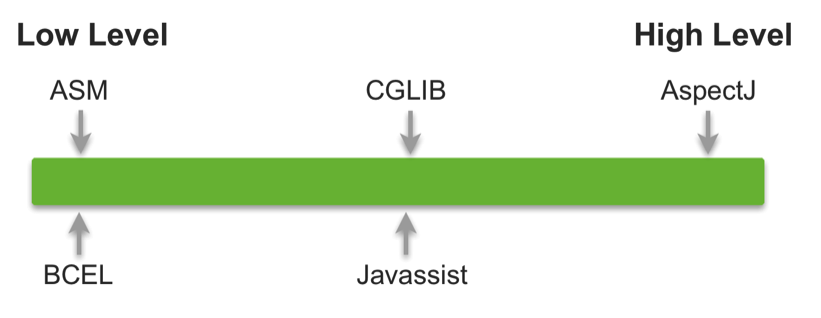
\includegraphics[width=0.8\linewidth]{javassistLevel}
%\caption{Bytecode modification levels.}
  %\label{fig:bytecodeModificationLevels}
%\end{figure}

%In \figref{bytecodeModificationLevels}\footnote{Figure taken from \href{https://blog.newrelic.com/2014/09/29/diving-bytecode-manipulation-creating-audit-log-asm-javassist/}{blog.newrelic.com}.} the term \textit{``Low Level''} is used for \textit{bytecode}-level and \textit{``High Level''} for \textit{source}-level. Using the libraries \textit{ASM} and \textit{BCEL} \brs{links or refs to these libs}the user has to construct bytecode itself and is not able to only write simple source code to modify a class file. The library \textit{AspectJ} on the other hand only allows the user to write source code which is than translated into bytecode. This way of course the user is limited by the functionality of the library \textit{AspectJ}. \textit{Javassist}\brs{not consistent, sometimes textit sometimes not. I don't see why it should be textit, I receomend droping it} and \textit{CGLIB} provide the user the choice of whether to work on \textit{bytecode}- or \textit{source}-level, or even on both. \brs{this whole story about ``levels'' is important because...}\lt{figure shows that javassist can use both apis.. take out?}

Let us look at the small example shown in \coderef{javassistExample}\footnote{Example taken from Javassist tutorial.} of how the bytecode manipulation with Javassist works. We go through the example line by line.

\renewcommand\lstlistingname{Code}
\begin{Java}[caption={Javassist example. With this example we explain how Javassist can be used.}, label={code:javassistExample}][H]
ClassPool pool = ClassPool.getDefault();
CtClass cc = pool.get("test.Rectangle");
cc.setSuperclass(pool.get("test.Point"));
cc.writeFile();
\end{Java}

\begin{enumerate}
	\item First a \textit{ClassPool} object that controls bytecode modification is obtained. With the \textit{ClassPool} object a class file (``.class'') can be read on demand for constructing a \textit{CtClass} object.

	\item The class \textit{CtClass} (compile-time class) represents the class file. This means that all manipulations are performed on the \textit{CtClass} object. We obtain a reference to the \textit{CtClass} object representing the \code{test.Rectangle} class by invoking the \code{get()} method on the \textit{ClassPool} instance.

	\item In this example the only bytecode modification done is changing the superclass of \code{test.Rectangle} to \code{test.Point}. This change serves only for illustration.

	\item Once the bytecode modification is done, the method call \code{writeFile()} on the instance of \textit{CtClass} is necessary to make sure that the changes are reflected on the original class file. The method \code{writeFile()} converts the modified \textit{CtClass} object into a class file and stores it on a local disk.
\end{enumerate}

\begin{figure}[H]
\centering
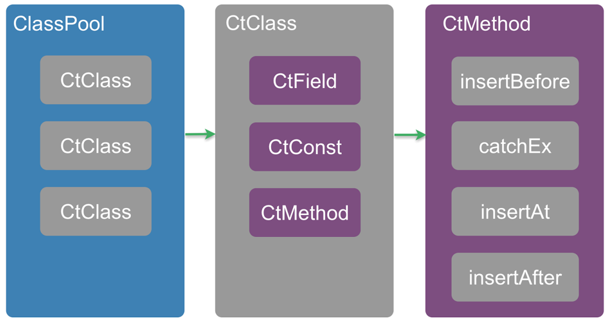
\includegraphics[width=0.8\linewidth]{javassistModules}
\caption{Javassist modules.}
  \label{fig:javassistModules}
\end{figure}

\figref{javassistModules}\footnote{Figure taken from \href{https://blog.newrelic.com/2014/09/29/diving-bytecode-manipulation-creating-audit-log-asm-javassist/}{blog.newrelic.com}.} gives an overview of how the main part of bytecode manipulation with Javassist is built up. The \textit{ClassPool} is simply a container of multiple \textit{CtClasses}. As described before \textit{CtClass} represents a class file on which modifications are done. Like typical classes, it can hold compile-time fields, constants or methods. Javassist is capable of adding or modifying classes, behaviors, fields, method invocations, local variables \etc But in our case we mainly address the manipulation of behaviors. It is possible to insert additional source code at the beginning of a method body, at the end or at a specific line. 

\renewcommand\lstlistingname{Code}
\begin{Java}[caption={Initial code.}, label={code:initialCode}][H]
public static void main(String[] args) {
	System.out.println("This is an example class.");
}
\end{Java}

\renewcommand\lstlistingname{Bytecode}
\begin{JVMIS}[caption={Initial bytecode.}, label={bytecode:initialBytecode}, numbers=left, breaklines=true][H]
public static void main(java.lang.String[]);
  0: getstatic     #16	// Field java/lang/System.out:Ljava/io/PrintStream;
  3: ldc           #22	// String This is an example class.
  5: invokevirtual #24	// Method java/io/PrintStream.println:(Ljava/lang/String;)V
  8: return
\end{JVMIS}

The next example (\coderef{bytecodeModifier}) shows how to add code by using Javassist.
We want to add one line of code at the beginning of the \code{main()} method in \coderef{initialCode}. \bytecoderef{initialBytecode} is the corresponding bytecode of \coderef{initialCode}.

\renewcommand\lstlistingname{Code}
\begin{Java}[caption={Bytecode modifier.}, label={code:bytecodeModifier}][H]
public class BytecodeModifier {
	public static void main(String[] args) ... {
		ClassPool pool = ClassPool.getDefault();
		CtClass cc = pool.get("insertJavaCodeExample.ExampleClass");

		CtBehavior behavior = cc.getDeclaredMethod("main");
		behavior.insertBefore("System.out.println(\"This is the inserted code.\");");

		cc.writeFile();
		...
	}
}
\end{Java}

We first obtain a \textit{CtClass} object \code{cc} (\coderef{bytecodeModifier} line 4) which represents the class to be modified. At line 6 we get the \textit{CtMethod} object \code{behavior} which represents the method we want to modify (in our case, method \code{main()}). We modify the method by adding the source code \code{System.out.println(``This is the inserted code.'');} at the beginning of the method. Because we want to insert code at the beginning of the method we invoke the method \code{insertBefore()} at line 7. If we wanted to enter additional code at the end of the method we could have called the analogue method \code{insertAfter()}. Both methods \code{insertBefore()} and \code{insertAfter()} expect an argument of type String, which Javassist then compiles, and adds into the bytecode at the specified location (in our situation at the beginning of the \code{main()} method).

If the modified bytecode (\bytecoderef{modifiedBytecode}) were to be decompiled, its source code representation is shown in the \coderef{modifiedCodeDecompiled}. A the line 2 of this code, we can see the changes, \ie the inserted line of code. But the actual result is the inserted bytecode represented by the pc-interval <0,5> in the modified bytecode (\bytecoderef{modifiedBytecode}).

\renewcommand\lstlistingname{Bytecode}
\begin{JVMIS}[caption={Modified bytecode. The modification is visible from line 0 to 4.}, label={bytecode:modifiedBytecode}, numbers=left, breaklines=true][H]
public static void main(java.lang.String[]);
  0: getstatic     #16 	// Field java/lang/System.out:Ljava/io/PrintStream;
  3: ldc           #35	// String This is the inserted code.
  5: invokevirtual #24	// Method java/io/PrintStream.println:(Ljava/lang/String;)V
  8: getstatic     #16	// Field java/lang/System.out:Ljava/io/PrintStream;
 11: ldc           #22	// String This is an example class.
 13: invokevirtual #24	// Method java/io/PrintStream.println:(Ljava/lang/String;)V
 16: return
\end{JVMIS}

\renewcommand\lstlistingname{Code}
\begin{Java}[caption={Modified code: Decompiled with JAD (\secref{jad})}, label={code:modifiedCodeDecompiled}][H]
public static void main(String args[]) {
	System.out.println("This is the inserted code.");
	System.out.println("This is an example class.");
}
\end{Java}

%===============================================================================
\section{JAD}
\label{sec:jad}

Java Decompier (JAD)\footnote{\url{https://sourceforge.net/projects/jadclipse/}} is a decompiler and an Eclipse plugin for the programming language Java. A decompiler is a program that takes an executable file as input, and attempts to create a high level, compatible source file. If the source file is compiled again, it will produce an executable program that behaves the same way as the original one. It is often used in software reverse engineering.

The example \bytecoderef{jad} is decompiled by JAD and the result is the source code shown in \coderef{decompiledBytecode}.

\renewcommand\lstlistingname{Bytecode}
\begin{JVMIS}[caption={This bytecode example serves as a demonstration code to be compiled with JAD.}, label={bytecode:jad}, breaklines=true]
public void itemStateChanged(java.awt.event.ItemEvent e);
  0  aload_1 [e]
  1  invokevirtual java.awt.event.ItemEvent.getStateChange() : int [23]
  4  iconst_1
  5  if_icmpne 22
  8  aload_0 [this]
  9  getfield org.jhotdraw.applet.DrawApplet$1.this$0 : org.jhotdraw.applet.DrawApplet [12]
 12  aload_1 [e]
 13  invokevirtual java.awt.event.ItemEvent.getItem() : java.lang.Object [29]
 16  checkcast java.lang.String [33]
 19  invokevirtual org.jhotdraw.applet.DrawApplet.loadDrawing(java.lang.String) : void [35]
 22  return
Line numbers:
 [pc: 0, line: 213]
 [pc: 8, line: 214]
 [pc: 22, line: 216]
Local variable table:
 [pc: 0, pc: 23] local: this index: 0 type: new org.jhotdraw.applet.DrawApplet(){}
 [pc: 0, pc: 23] local: e index: 1 type: java.awt.event.ItemEvent
\end{JVMIS}

\renewcommand\lstlistingname{Code}
\begin{Java}[caption={The result of the decompiled bytecode shown in \bytecoderef{jad}.}, label={code:decompiledBytecode}]
public void itemStateChanged(ItemEvent e) {
	if(e.getStateChange() == 1)
		loadDrawing((String)e.getItem());
}
\end{Java}
 
JAD is in no way a dependency of NullSpy but it was a big help during the implementation phase since after running NullSpy on a project only the modified bytecode is available. The use of JAD is for the sake of debugging NullSpy; to check whether the modification made by Javassist, \ie inserting source code, was successful. Another way to check the result for correctness is looking at bytecode itself but that would have taken a lot more effort and time.

%%%%%%%%%%%%%%%%%%%%%%%%%%%%%%%%%%%%%%%%%%%%%%%%%%%%%%%%%%%%%%%%%%%%%%%%%%%%%%%%
%                                   NullSpy                                    %
%%%%%%%%%%%%%%%%%%%%%%%%%%%%%%%%%%%%%%%%%%%%%%%%%%%%%%%%%%%%%%%%%%%%%%%%%%%%%%%%
\chapter{NullSpy}

As explained in \charef{introduction}, this project is about providing the user with an additional link next to the common stack trace containing the location of a \textit{null} assignment to the variable that caused the \npe. We use the term \textbf{link} to address the line which includes the information where the variable that caused the \npe was assigned null, and which we add to the common stack trace.

In this chapter we give an overview of how we implemented NullSpy. We will also address the challenges (\secref{challenges}) we encountered during the implementation as well as the limitations of the tool (\secref{limitations}).

%===============================================================================
\section{High Level Overview}
\label{sec:highLevelOverview}

The general approach of NullSpy is to statically analyze a project in which \npe occurs and instrument the corresponding bytecode. NullSpy is a console application which takes two arguments. The first argument to NullSpy is the local path to the folder containing the compiled class files of the original project and the second one is the path to the folder in which the user wants to store the modified class files.

We provide the option to choose the destination in case the developer does not want to overwrite the original project with the modified one. This means that the updated bytecode can be stored in another location, keeping the original class files intact. Of course the original project can also be replaced by the modified one. To sweep away the instrumented bytecode, the developer has to recompile the source code to get the original class files when needed.

\begin{figure}[H]
\centering
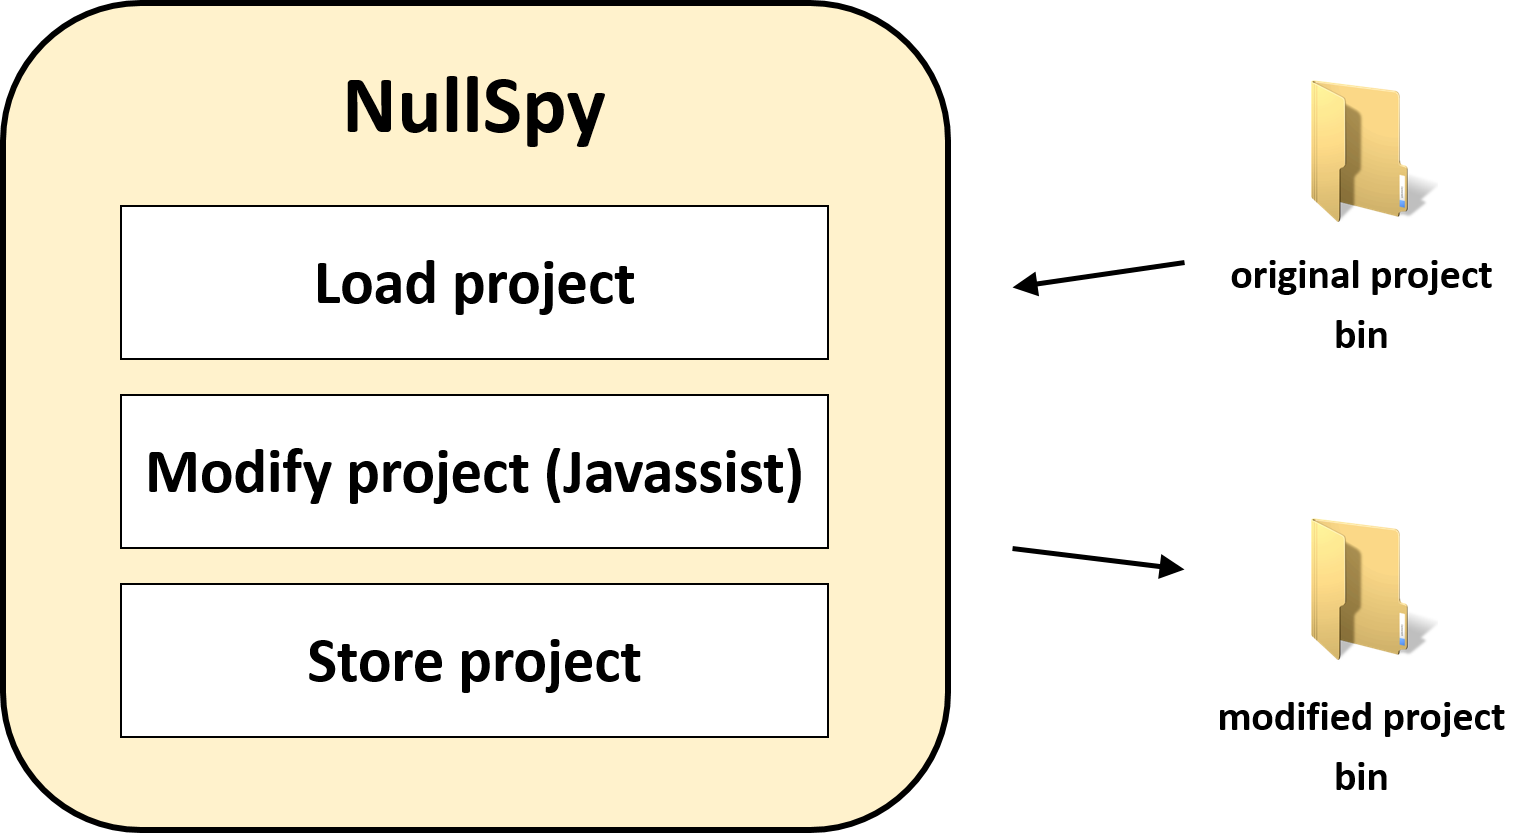
\includegraphics[width=0.8\linewidth]{highLevelOverview3}
\caption{High level overview.}
  \label{fig:highLevelOverview}
\end{figure}

NullSpy contains three basic steps which we can see in \figref{highLevelOverview}: \textit{load, modify, store}. Those three steps of NullSpy carry out the following actions:

\begin{enumerate}
	\item Input: Load compiled class files of the project into NullSpy.
	\item Modification: The modification part deals with the bytecode instrumentation and adding modules to the project that support the inserted code.
	\item Output: Store modified class files to the chosen output folder.
\end{enumerate}

Loading is done by traversing through all the subfolders of the folder whose local path was given as a first parameter, and extracting all the \textit{.class} files. NullSpy modifies the class file directly when it is loaded. As soon as the modification is done, the class file is stored at the destination folder \ie the folder whose path is the second parameter of NullSpy. The structure of the source folder is preserved also at the destination folder.

%\chg{Storing is done by recreating the structure from the source folder in the destination folder. \ugh{and storing the modified class files.  using the Javasist API.}}{The structure of the source original folder is preserved also at the destination folder.} \nm{I would not mention JavaAssist here, no need for it.}

%\del{In secref{javassist} we store the modified class file on a local disk. This way the original class file remains intact. In our case we write the modified class file in the destination folder not only on a local disk. This way the original project can be overwritten as explained before.} \brs{what? not only on a local disk? what does that even mean}\lt{ask, javassist tutorial store on local disk, here write new file or overwrite}

%===============================================================================
\section{Low Level Overview}
\label{sec:lowLevelOverview}

In this section we will focus on the bytecode modification. \figref{modificationModules} shows that the modification part of NullSpy contains three different modules. Each class file of the loaded project will be run through the first two modules and the last module is only added once to the modified project at the end of the instrumentation process.

After class loading, we first extract data from the class bytecode and then instrument it.

\begin{figure}[H]
\centering
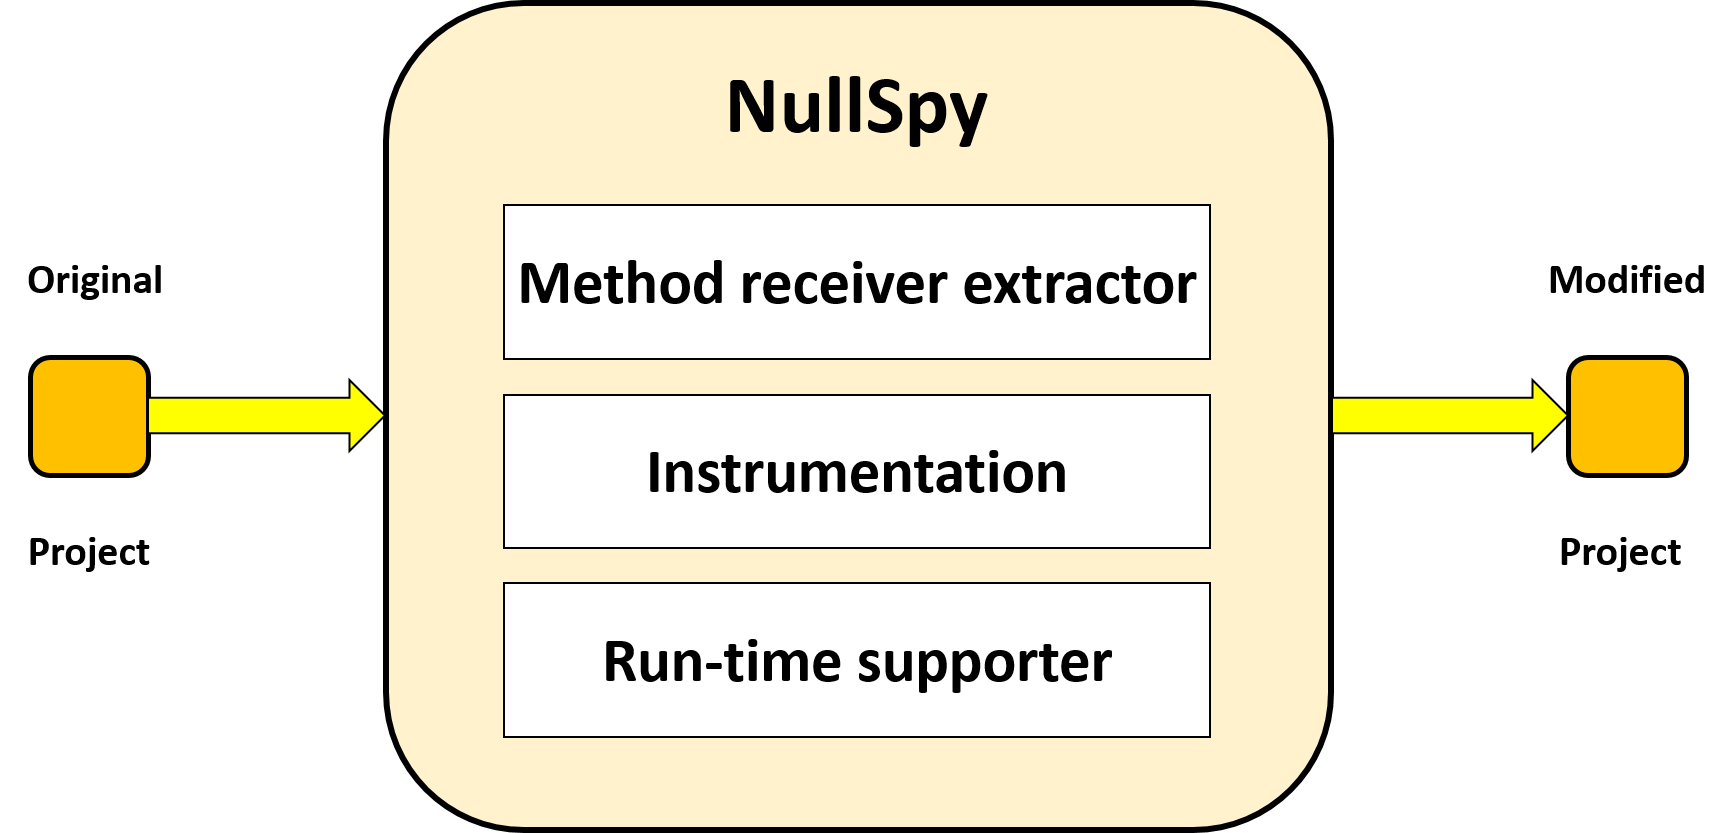
\includegraphics[width=0.8\linewidth]{lowLevelOverview}
\caption{NullSpy modification modules.}
  \label{fig:modificationModules}
\end{figure}

We will look at these modules in more detail and explain what each one does.

%-------------------------------------------------------------------------------
\subsection{Process Flow}
\label{subsec:processFlow}
In this short and rough overview of the entire process we explain the reason why we have to extract data from bytecode and what they are used for. Details are discussed in the following subsections.

From the stack trace of a \npe we can obtain three kinds of information: the class name, method name and the line number of where the \npe happened. The aim of NullSpy is to reveal the location of the null assignment to the variable which caused the \npe. To achieve this goal we need to take information from the bytecode about \textbf{\mrs} and \textbf{null assignments}.

The first step in the modification part is to statically gather information about the \mrs. We use the term \textbf{\mr} to refer to variables on which methods are invoked, or whose fields are accessed.
These variables are candidates for triggering a \npe.
For each \mr we extract the information needed to create its unique identifier (details about this are listed in \subsecref{methodReceiver}). 
These identifiers are used later to track the assignments to the aforementioned variable, and to find the null assignment entry for this variable, if any.

The second step is to instrument the assignments. For every non-primitive variable assignment we collect information about the variable, needed to create its unique identifier. After the assignment we insert code which represents a call to the \textbf{run-time supporter} package with the variable's identifier. The run-time supporter package checks at run-time whether the variable is assigned null. If this is the case we store the information about this variable.

At the end of the bytecode modification part we wrap the \code{main()} method into a \tcblock. This \tcblock extract from the \npe stack trace the information about the location where the exception happened (class name, method name, line number). This is the only information we can get from a stack trace. This information is passed on to the run-time supporter package which compares it with the stored identifiers about the \mrs. If there is a match regarding the comparison, NullSpy uses this identifier to reveal the information stored about the assignments to this variable. If there is an entry about the null assignment of that variable, we extract from it the line number of the assignment and create the additional link that reveals the location of the null assignment. This link is then added to the common \npe stack trace.

%\brs{everything in this subsection after this point makes no sense to me. ``As soon as a \npe is thrown'' how do we know when it's thrown? ``sequentially compare data'' what does this even mean?}
%
%\chk{To summarize the last three paragraphs:
%As soon as a \npe is thrown, we extract data from the \npe stack trace and information about the \mr and the null assignments. We then sequentially compare those data with each other to get the right location of the null assignment.} The comparison-sequence looks as follows (we use the symbol ``\textbf{$\|$}'' for the comparison):
%
%\begin{enumerate}
	%\item \npe data \textbf{$\|$} \mrs data $\rightarrow$ \mr-identifier
	%\item \mr-identifier \textbf{$\|$} null assignment data $\rightarrow$ \textbf{result}
%\end{enumerate}
%
%Result contains the data needed to create the link to the null assignment.
%
%Finally we add the \textit{run-time supporter} module to the modified project.

The way how we extract and store all those data are discussed in the following sections.

%-------------------------------------------------------------------------------
\subsection{\MR Data Collection}
\label{subsec:methodReceiver}
In this section we explain how to get information about the \mr needed to construct a unique identifier. \Mrs in the example \coderef{methodReceiverAlgDemoCode} are the variables \code{fToolButton} at line 7, \code{fToolButton.myIcon} at line 8 and \code{activePanel} at line 11.

We use the library Javassist to partially extract this data from bytecode. Unfortunately, Javassist does not provide the functionality to directly get all the information we need about the \mr, thus we need to do it manually. 

\renewcommand\lstlistingname{Code}
\begin{Java}[caption={Code snippet to demonstrate the \mr extracting algorithm.}, label={code:methodReceiverAlgDemoCode}]
public class DrawApplication {

	private ToolButton fToolButton;

	protected void open(final DrawingView newDrawingView) {
	...
	(@\textbf{fToolButton}@).tool();			   // field access
	(@\textbf{fToolButton.myIcon}@).toString();	// field access
		
	JPanel activePanel = new JPanel();		
	(@\textbf{activePanel}@).add((Component) getDesktop(), BorderLayout.CENTER);	// local variable as a method receiver
	...
	}
}
\end{Java}

\renewcommand\lstlistingname{Bytecode}
\begin{JVMIS}[numbers=left, caption={Bytecode of \coderef{methodReceiverAlgDemoCode}.}, label={bytecode:methodReceiverAlgDemoBytecode}, breaklines=true]
144  aload_3 [activePanel]
145  aload_0 [this]
146  invokevirtual org.jhotdraw.application.DrawApplication.getDesktop() : org.jhotdraw.contrib.Desktop [271]
149  checkcast java.awt.Component [274]
152  ldc_w <String "Center"> [276]
155  invokevirtual javax.swing.JPanel.add(java.awt.Component, java.lang.Object) : void [254]
\end{JVMIS}

\textbf{Finding the invocation opcode/end-pc}\\
Let us suppose that we are interested in the \mr \code{activePanel} of the method invocation \code{add(...)} at line 11 in the example \coderef{methodReceiverAlgDemoCode}.
Its bytecode is presented in \bytecoderef{methodReceiverAlgDemoBytecode}.

To get data about \mrs we iterate through the bytecode looking for the instructions which represent a method invocation.
To do this, NullSpy looks for the opcodes which matches the regex \textit{``invoke.*''}. Each of these opcodes represents one method invocation. There are exactly five invocation bytecode instructions in Java: \textit{invokedynamic}, \textit{invokeinterface}, \textit{invokespecial}, \textit{invokestatic}, \textit{invokevirtual}.

For each method invocation we want to find the method receiver. 
In our example bytecode instruction which matches the invocation of the method \code{add(...)} is at the line 6 in \bytecoderef{methodReceiverAlgDemoBytecode}.
Since bytecode lists method receiver and all the method parameters before the \textit{``invoke.*"} instruction, the pc of this \textit{``invoke.*''} opcode will represent the \textbf{end-pc} of the method invocation pc-interval. In our example, the end-pc of the method invocation \code{add(...)} is 155.

\textbf{Finding the start-pc}\\ 
The \textbf{start-pc} of the method invocation pc-interval is the pc at which begins the bytecode which represents the source code line, containing the invocation. Finding the start-pc is done by using the line number table of the method. We compare the \textbf{end-pc} with the entries of the line number table and take the last entry which has the smaller pc than the \textbf{end-pc}. The line number table of the example bytecode is shown in \bytecoderef{mrBytecodeExampleLineNumberTable}. 
The \textbf{start-pc} in our example is 144.

\renewcommand\lstlistingname{Bytecode}
\begin{JVMIS}[caption={Part of the line number table of the example bytecode shown in \bytecoderef{methodReceiverAlgDemoBytecode}.}, label={bytecode:mrBytecodeExampleLineNumberTable}, breaklines=true]
Line numbers:
	...
	[pc: 136, line: 10]
	(@\textbf{[pc: 144, line: 11]}@)
	[pc: 158, line: 12]
	...
\end{JVMIS}

We define the outermost \textbf{pc-interval} as the interval starting with the \textbf{start-pc} and ending with the \textbf{end-pc}. We know that the \mr is located in this interval. In our example, this is <144,155>.

\textbf{Extracting candidate \mr pc-intervals}\\
The outermost interval <144,155> could contain other invocations, which could have \mrs of their own. This is visible in our example, where the \code{getDesktop()} invocation (pc 146) is embedded in our outermost interval. For this reason, we explored all possible bytecode combinations of instructions that can represent \mrs and developed a system for identifying such embedded call sights. More about this system can be found in the Appendix (\ref{cha:bytecodeCombinations}). This system allows us to split the outermost pc-interval into candidate \mr pc-intervals. In our example, the outermost pc-interval is divided into \{<144,144>,<145,149>,<152,152>\}. Each of the pc-intervals represents:

\begin{enumerate}
	\item <144,144>: variable \code{activePanel}
	\item <145,149>: first parameter \code{(Component) getDesktop()}
	\item <152,152>: second parameter \code{BorderLayout.CENTER}
\end{enumerate}

\textbf{Finding the actual \mr}\\
The set of candidate pc-intervals ends with the arguments of the method.
Javassist allows us to obtain the number of parameters of a method invocation by analyzing the method signature. 
Thus, if the method expects $N$ arguments, we can ignore the last $N$ candidate pc-intervals. The one before them is the actual \mr pc-interval. 
In our example, since the method takes two arguments, the actual \mr pc-interval is <144,144>.

If the \mr is actually return object from another method invocation, it is unapparent where exactly the \mr is situated in bytecode. More about the challenges we encountered can be found in \subsecref{methodReceiverDifficulties}.

In case of the simple stand-alone \textit{invokestatic} instruction we do have a \mr but NullSpy ignores these instructions because static method invocations are called on classes which can never be null. But if the static method call is a parameter of another method call, NullSpy still treats it as a \mr candidate. As for the other \textit{invoke} instructions, they are treated normally as explained.

With the \mr pc-interval we extract the information needed to create a unique \mr identifier from the bytecode by using Javassist API.
We get the index of the \mr by using Javassist (in our example the index is 3), and with this index and pc information of the \mr, we can obtain the needed information from the local variable table shown in \bytecoderef{mrBytecodeExampleLocalVariableTable}.

\renewcommand\lstlistingname{Bytecode}
\begin{JVMIS}[caption={Part of the local variable table of the example bytecode shown in \bytecoderef{methodReceiverAlgDemoBytecode}.}, label={bytecode:mrBytecodeExampleLocalVariableTable}, breaklines=true]
Local variable table:
	...
	[pc: 100, pc: 340] local: activePanel index: 3 type: javax.swing.JPanel
	...
\end{JVMIS}

The next listing shows a part of the extracted information about the \mr to create its unique identifier:
\begin{itemize}
	\item source code line number of the method receiver
	\item name of the class and signature of the method containing the method invocation
	\item full variable name
	\item statically declared variable type
\end{itemize}

The exact information we need can be found in the Appendix \ref{cha:appReceivers}.

%-------------------------------------------------------------------------------
\subsection{Assignments Collection}
\label{subsec:variable}

%In the precious section we were looking for instructions which match the regex \textit{``invoke.*''} to detect \mrs in bytecode. 
To find the assignments in the bytecode we search for the instructions matching regexs \textit{``astore.*''} and \textit{``put.*''}. The former refers to local variable assignments and the latter to field assignments. 
%Unlike the information collection of the \mr, the data about the variables are stored in a HashMap, since it needs to be used at run time.

In the next two subsections we will look at how the information about the assigned variables is extracted. Due to different variable types and the limitation of Javassist, the ways of gathering information about the local variables and fields are performed differently.

\subsubsection{Local Variable}
\label{subsubsec:localVariable}
Unfortunately, Javassist does not provide any support for gaining information about local variables, thus we needed to do it manually. 
%This is why we have to understand how the bytecode is constructed concerning the local variables. 
%In \secref{bytecode} we introduced the parts of the bytecode that are important for our project NullSpy.

%We have to pay attention to get the right local variable every time we encounter one while iterating through bytecode. 
Every time we hit upon the opcode \textit{``astore.*''}  (which represents an assignment to a local variable) we get the index of the variable and the pc of the assignment instruction. A local variable has a limited lifespan. As we have already seen in \secref{bytecode} multiple entries can have the same local variable slot (one variable takes the index of the other whose lifespan expired).

\begin{JVMIS}[numbers=left, caption={Local variable table entries with same slot 2 (line 4 and7).}, label={bytecode:localVarTableDuplicatedSlot}, breaklines=true]
Local variable table:
 [pc: 0, pc: 95] local: this index: 0 type: org.jhotdraw.samples.javadraw.JavaDrawViewer
 [pc: 0, pc: 95] local: filename index: 1 type: java.lang.String
 (@\textbf{[pc: 13, pc: 40] local: url index: 2 type: java.net.URL}@)
 [pc: 18, pc: 40] local: stream index: 3 type: java.io.InputStream
 [pc: 28, pc: 40] local: reader index: 4 type: org.jhotdraw.util.StorableInput
 (@\textbf{[pc: 44, pc: 94] local: newTool index: 2 type: org.jhotdraw.framework.Tool}@)
\end{JVMIS}

\begin{JVMIS}[numbers=left, caption={Local variable assignment at pc 45.}, label={bytecode:localVarAssignment}, breaklines=true]
Local variable table:
	...
	37  aload_0 [this]
	38  invokevirtual org.jhotdraw.samples.javadraw.JavaDrawViewer.getCodeBase() : java.net.URL [100]
	41  aload_1 [filename]
	42  invokespecial java.net.URL(java.net.URL, java.lang.String) [104]
	(@\textbf{45  astore\_2 [url]}@)
	...
\end{JVMIS}
    
Let us assume that we have a local variable assignment where its \textit{``astore\_2''} opcode is located at pc 45 (\bytecoderef{localVarAssignment}). In this example we can extract slot 2 from the opcode \textit{astore\_2}. After extracting the slot (index: 2) we iterate through the local variable table and find the first entry which contains that slot (line 4 in \bytecoderef{localVarTableDuplicatedSlot}). If the pc of the assignment is not included in the local variable lifespan of the entry (pc 45 $\notin$ [pc: 13, pc: 40], line 4), the next entry with the same slot (pc 45 $\in$ [pc: 44, pc: 94], line 7) will be examined. Checking the entries with the same slot goes on until both criteria slot and pc fits. Once those criteria are met we can be positive about having the right local variable table entry to extract the information needed to create a unique identifier for the variable. We now extract from local variable table the information we need to create a unique identifier for a variable. A part of the extracted information is listed below:
\begin{itemize}
	\item source code line number of the assignment
	\item name of the class and method signature containing the local variable
	\item local variable name
	\item statically declared local variable type
\end{itemize}

The exact list of the information we extract can be found in the Appendix \ref{cha:appLocalVars}.

\begin{JVMIS}[numbers=left, caption={Line number table.}, label={bytecode:lineNrTable}]
  Line numbers:
        [pc: 0, line: 58]
        [pc: 13, line: 59]
        [pc: 18, line: 60]
        [pc: 28, line: 61]
        [pc: 40, line: 62]
        [pc: 43, line: 63]
        (@\textbf{[pc: 44, line: 64]}@)
        [pc: 52, line: 65]
        [pc: 74, line: 66]
        [pc: 94, line: 68]
\end{JVMIS}

On the other hand, by using the pc of the assignment (45) and line number table (shown in \bytecoderef{lineNrTable}) we obtain the source code line number of the assignment. As we can see in the table, the local variable assignment starts at source code line 64.

\subsubsection{Instance and Class/Static variable (Field)}
\label{subsubsec:field}
Although Javassist does not support the access to information about local variables it provides a way to access information about fields. Javassist allows us to modify an expression in a method body by using the class \code{Javassist.expt.ExprEditor}. 
%In our case we only want to extract some information about the fields instead of any modification, nevertheless this class can be used appropriately. 
It scans the bytecode for instructions like \textit{``putfield''} for instance fields or \textit{``putstatic''} for static fields, and allows us to directly get the information we need to create a unique identifier for the field. Next we list a part of the information we are interested in:
\begin{itemize}
	\item source code line number of the assignment
	\item name of the class and method signature containing the field assignment
	\item full field name
	\item statically declared field type
\end{itemize}

During the data collection about the fields we encountered some difficulties which we will discuss in \subsecref{variableDifficulties}.

As already mentioned earlier, every time when encountering an assignment either to a local variable or a field, NullSpy inserts bytecode which checks at run time whether the variable is assigned null. If the variable is assigned null, NullSpy stores all the data about the variable.

%-------------------------------------------------------------------------------
\subsection{Bytecode Adaptation}
\label{bytecodeAdaptation}
Each time we encounter a variable assignment we first extract the data about the variable and then we add our own bytecode right after the assignment bytecode. The inserted bytecode checks at run time whether the value being assigned to the variable is null. If this is the case, we store the previously explained information about this assignment.

The explanation of the way we do it can be found in the Appendix \ref{cha:appInstrumentation}.

Once we have gone through the bytecode of all the class files, the modified class files are stored in the destination directory as mentioned in \secref{highLevelOverview}. After the instrumentation we add out supplementary supporter classes to the project. The most important ones are \code{VariableTester}\footnote{\label{package1}In package \emph{ch.scg.nullSpy.runtimeSupporter}} which tests whether a variable is null and \code{NullDisplayer}\textsuperscript{\ref{package1}} which matches data and prints the location of a null assignment when a \npe is thrown.

%===============================================================================
\section{Challenges}
\label{sec:challenges}

In this section we would like to present some of the difficulties we encountered during the implementation of NullSpy.

%-------------------------------------------------------------------------------
\subsection{Obtaining \MR Data Difficulties}
\label{subsec:methodReceiverDifficulties}

In the section \subsecref{methodReceiver} we have explained how to extract the information about \mr when the whole method invocation is contained within one line of code. 
%In many development environment the written code can be formatted automatically and as well manually. 
However, we have encountered a persistent problem, namely getting the pc-interval of the \mr when the method invocation is split throughout multiple lines of code, thus when method invocation pc-interval covers multiple lines in source code.  

\renewcommand\lstlistingname{Code}
\begin{Java}[caption={Method invocation split in two lines example.}, label={code:4-1}, firstnumber=31]
Image image = Iconkit.instance().registerAndLoadImage(
	(Component)view, imageName);
\end{Java}
%Class: org.jhotdraw.samples.minimap.MiniMapDesktop
%Method: createRightComponent

%\renewcommand\lstlistingname{Bytecode}
%\begin{JVMIS}[caption={Bytecode to \coderef{4-1}.}, label={bytecode:4-2}, breaklines=true]
 %0  invokestatic org.jhotdraw.util.Iconkit.instance() : org.jhotdraw.util.Iconkit [22]
 %3  aload_1 [view]
 %4  checkcast java.awt.Component [28]
 %7  aload_0 [this]
 %8  getfield org.jhotdraw.samples.minimap.MiniMapDesktop.imageName : java.lang.String [14]
%11  invokevirtual org.jhotdraw.util.Iconkit.registerAndLoadImage(java.awt.Component, java.lang.String) : java.awt.Image [30]
%14  astore_2 [image]
%\end{JVMIS}

\renewcommand\lstlistingname{Bytecode}
\begin{JVMIS}[numbers=left, caption={Line number table of \coderef{4-1}.}, label={bytecode:4-3}, breaklines=true, firstnumber=1]
Line number table:
	(@\textbf{[pc: 0, line: 31]}@)
	[pc: 3, line: 32]
	(@\textbf{[pc: 11, line: 31]}@)
	...
\end{JVMIS}

Let us now have a look at an example that contains the explained situation, where a method invocation is split into two lines. The example is shown in \coderef{4-1}. 
In this example we are interested in the method invocation \code{registerAndLoadImage(...)}. 
The invocation starts at line 31 and ends at line 32.
The second line only contains the arguments of the method call.
These situations cannot be figured out by just looking at the bytecode, therefore the line number table (\bytecoderef{4-3}) has to be consulted. 

Beforehand we have to say that there is no \mr (in the terms we defined it) in \coderef{4-1} because the \mr would be a method invocation itself. NullSpy does not support \mrs which are return objects of method invocations. Enabling the coverage of such situations is a part of the future work. Other \mrs NullSpy does not support are elements of collections since a collection can hold other collections, \etc

The line number \textit{31} is listed twice int the line number table (\bytecoderef{4-3}). This indicates that the method invocation is split into multiple lines in source code.

The line number table entries indicate the followings:
\begin{itemize}
	\item line 2: execution of the static method invocation \code{Iconkit.instance()}
	\item line 3: starting point where the parameters are loaded onto the operand stack
	\item line 4: execution of the method \code{registerAndLoadImage(...)}
\end{itemize}

To obtain the method invocation pc-interval we had to make further analyses. By using the algorithm described in \subsecref{methodReceiver} we would get <0,0> as the method invocation pc-interval, which is incorrect. The correct method invocation pc-interval in this example is <0,11>.

\renewcommand\lstlistingname{Code}
\begin{Java}[caption={Alternating line number example.}, label={code:3-1}, firstnumber=127]
Connector oldConnector = ((ChangeConnectionHandle.UndoActivity)
			getUndoActivity()).getOldConnector();
\end{Java}
%Class: org.jhotdraw.standard.ChangeConnectionHandle
%Method: invokeEnd

%\renewcommand\lstlistingname{Bytecode}
%\begin{JVMIS}[caption={Bytecode to \coderef{3-1}.}, label={code:3-2}, breaklines=true]
%47  aload_0 [this]
%48  invokevirtual org.jhotdraw.standard.ChangeConnectionHandle.getUndoActivity() : org.jhotdraw.util.Undoable [72]
%51  checkcast org.jhotdraw.standard.ChangeConnectionHandle(@\$@)UndoActivity [76]
%54  invokevirtual org.jhotdraw.standard.ChangeConnectionHandle(@\$@)UndoActivity.getOldConnector() : org.jhotdraw.framework.Connector [142]
%57  astore 7 [oldConnector]
%\end{JVMIS}

\renewcommand\lstlistingname{Bytecode}
\begin{JVMIS}[caption={Line number table/interval to \coderef{3-1}.}, label={bytecode:3-3}, breaklines=true, numbers=left]
Line number table:
	...
	[pc: 47, line: (@\textbf{128}@)]
	[pc: 51, line: (@\textbf{127}@)]
	[pc: 54, line: (@\textbf{128}@)]
	[pc: 57, line: (@\textbf{127}@)]
	...
\end{JVMIS}

More complicated situation as the one shown in the example \coderef{3-1} can happen. In this example method invocation is situated in the second line unlike the invocation in the previous example. This is interesting because the line numbers 127 and 128 are stored in an alternated way in the line number table shown in \bytecoderef{3-3}. The line number table indicates followings:

\begin{itemize}
	\item line 3: the method invocation \code{getUndoActivity()}
	\item line 4: the cast to \code{ChangeConnectionsHandle.UndoActivity}
	\item line 5: the second method invocation \code{getOldConnector()}
	\item line 6: the assignment to the variable \code{oldConnector}
\end{itemize}

First, the method invocation \code{getUndoActivity()} at line 128 is executed and then the execution jumps back to line 127 to perform the cast to \code{ChangeConnectionsHandle.UndoActivity}. After the cast, again execution jumps to line 128 where the method \code{getOldConnector()} is invoked.

With the default analyses we would obtain <47,48> as the invocation pc-interval, whereas the correct one is <47,54>. 
Another interesting thing is that the start-pc of the invocation is mapped to line 128. So the invocation does not start with the smaller line number, \ie line 127 what normally would be expected.

\renewcommand\lstlistingname{Code}
\begin{Java}[caption={Nested interval example.}, label={code:2-1}, firstnumber=149]
for (int i = 0; i < ColorMap.size(); i++)
	choice.addItem(
		new ChangeAttributeCommand(
			ColorMap.name(i),
			attribute,
			ColorMap.color(i),
			this
		)
	);
\end{Java}
%Class: org.jhotdraw.applet.DrawApplet
%Method: createColorChoice

%\renewcommand\lstlistingname{Bytecode}
%\begin{JVMIS}[caption={Bytecode to \coderef{2-1}.}, label={code:2-2}, breaklines=true]
 %8  iconst_0
 %9  istore_3 [i]
%10  goto 37
%13  aload_2 [choice]
%14  new org.jhotdraw.standard.ChangeAttributeCommand [213]
%17  dup
%18  iload_3 [i]
%19  invokestatic org.jhotdraw.util.ColorMap.name(int) : java.lang.String [246]
%22  aload_1 [attribute]
%23  iload_3 [i]
%24  invokestatic org.jhotdraw.util.ColorMap.color(int) : java.awt.Color [252]
%27  aload_0 [this]
%28  invokespecial org.jhotdraw.standard.ChangeAttributeCommand(java.lang.String, org.jhotdraw.framework.FigureAttributeConstant, java.lang.Object, org.jhotdraw.framework.DrawingEditor) [222]
%31  invokevirtual org.jhotdraw.util.CommandChoice.addItem(org.jhotdraw.util.Command) : void [225]
%34  iinc 3 1 [i]
%37  iload_3 [i]
%38  invokestatic org.jhotdraw.util.ColorMap.size() : int [256]
%41  if_icmplt 13
%\end{JVMIS}

\begin{JVMIS}[numbers=left, caption={Line number table/interval to \coderef{2-1}.}, label={bytecode:2-3}, breaklines=true]
Line number table:
	...
	[pc: 8, line: 149]
	[pc: 13, line: 150]
	[pc: 14, line: 151]
	[pc: 18, line: 152]
	[pc: 22, line: 153]
	[pc: 23, line: 154]
	[pc: 27, line: 155]
	[pc: 28, line: 151]
	[pc: 31, line: 150]
	[pc: 34, line: 149]
	...
\end{JVMIS}

The third situation we encountered is presented in the example (\coderef{2-1}). In the line number table, there are several pairs of entries corresponding to the same source code line number (line number table shown in \bytecoderef{2-3}), \ie lines 3 and 12 both correspond to the source code line 149, lines 4 and 11 both correspond to the source code line number 150 and lines 5 and 10 both correspond to the source code line 151. 
The first line of these pairs indicates the start-pc of an expression and the latter represents the end-pc of the expression. Again, we examine the line number table:

\begin{enumerate}
	\item line 3: start-pc of the for-loop
	\item line 4: start-pc of the method invocation \code{addItem(...)}
	\item line 5: \code{new ChangeAttributeCommand(...)} start-pc\\which is actually argument loading onto the stack
	\item line 6-8: argument loading onto the operand stack
	\item line 9-10: object creation \code{new ChangeAttributeCommand(...)}
	\item line 11: call to \code{addItem(...)}
	\item line 12: for-loop incrementation
\end{enumerate}

%\renewcommand\lstlistingname{Code}
%\begin{Java}[caption={Incomplete interval example.}, label={code:5-1}, firstnumber=22]
%var_1
	%.method_1(staticMethod_1(),
		%staticMethod_2(param_1),
		%var_2.method_2(null,
			%param_2));
%\end{Java}

%\renewcommand\lstlistingname{Bytecode}
%\begin{JVMIS}[caption={Bytecode to \coderef{5-1}.}, label={code:5-2}, breaklines=true]
%18  aload_1 [var_1]
%19  invokestatic staticMethod_1() : java.lang.Object [26]
%22  aload_3 [param_1]
%23  invokestatic staticMethod_2(java.lang.Object) : java.lang.Object [30]
%26  aload_2 [var_2]
%27  aconst_null
%28  aload_3 [param_2]
%29  invokevirtual method_2(java.lang.Object, java.lang.Object) : java.lang.Object [34]
%32  invokevirtual method_1(java.lang.Object, java.lang.Object, java.lang.Object) : void [38]
%\end{JVMIS}

%\begin{JVMIS}[caption={Line number table/interval to \coderef{5-1}.}, label={code:5-3}, breaklines=true]
%[pc: 18, line: 22]
%[pc: 19, line: 23]
%[pc: 22, line: 24]
%[pc: 26, line: 25]
%[pc: 28, line: 26]
%[pc: 29, line: 25]
%[pc: 32, line: 23]
%\end{JVMIS}

By using the algorithm of extracting the pc-interval of a \mr (described in \subsecref{methodReceiver}) we would again get the wrong outermost pc-interval of the method invocation. To handle this mistake we implemented a supporting class called \code{MultipleLineManager}\footnote{In package \emph{ch.unibe.scg.nullSpy.instrumentator.controller.methodInvocation}.}. Its responsibility is to extract the outermost pc-interval of invocations in split line situations. 
For complexity reasons we omit the implementation explanation.

%only get the pc-interval <47,>, but actually pc 18 also belongs to the interval. That the missing pc is missing will be detected in step 4\&5 when traversing back the ArrayList by the number of parameters. If it is not a static method invocation and there is not enough possible \mrs stored in that ArrayList to traverse back, the missing pc is added in retrospect.
%
%\renewcommand\lstlistingname{Pseudocode}
%\begin{Java}[caption={Multiple line interval algorithm.}, label={alg:multipleLineAlg}]
%i = index in line number attribute which contains the invoke.* opcode
%
%if (lineNrAttribute[j>i] <= lineNrAttribute[i]) {
%
	%if (isAlternating(i,j))
		%return getAlternatingInterval(i, j);
%
	%// non-alternating
	%b = j which has the smallest line number after j;
	%a = corresponding index to b; // index<k which has the same line number as b||k
	%return getNonAlternatingInterval(a, b);
%
%} else if (lineNrAttribute[j<i] == lineNrAttribute[i]) {
%
		%b = i;
		%a = j;
		%return getInterval(a, b);
%
%}
%\end{Java}
%
%This pseudocode will give a very rough idea how the invocation interval can be read out. The detailed implementation can be seen in the classes \code{MultipleLineManager}\footnote{\label{package2}In package \emph{ch.unibe.scg.nullSpy.instrumentator.controller.methodInvocation}.} and \code{MethodInvocationAnalyzer}\textsuperscript{\ref{package2}}.

%-------------------------------------------------------------------------------
\subsection{Obtaining Assignment Data Difficulties - Fields}
\label{subsec:variableDifficulties}

\nm{Boris, could you have a look at this? We need to discuss this on Tuesday.}

We mentioned that NullSpy collects data about fields with help of the class \code{Javassist.expt.ExprEditor}. This class uses the method \code{loopBody(...)} to iterate through bytecode of a method and scans for specific opcodes, in our place we are only interested in the opcodes which matches the regex \textit{``put.*''}. One parameter passed to the method \code{loopBody(...)} is the \code{mehodInfo} object which contains the bytecode of the method we want to instrument.

Since the \code{loopBody(...)} is invoked within a \code{while-loop}, it iterates through the given \code{methodInfo} until it reaches the end of the bytecode sequence. When it goes through the bytecode sequence we instrument the bytecode. But because the changes made on the bytecode is updated after the \code{while-loop}, the method \code{loopBody(...)} still finds the specific opcodes at locations within the origin bytecode sequence instead of the modified one.

Due to this situation we had difficulties finding the right \textbf{start-pc} of field assignments. The class \code{FieldAnalyzer}\footnote{In package \emph{ch.unibe.scg.nullSpy.instrumentator.controller}.} serves as the explanation of how we still managed to find the \textbf{start-pc} of a field assignment.

%This method caused us some.  troubles because it loops through the GIVEN \code{methodInfo} which contains the bytecode sequence of a method. Even after finding a field assignment and adding bytecode to it, the method still iterates through the unchanged \code{methodInfo} it got as parameter without the additional bytecode. Getting the right start-pc of a field assignment is not a straight forward process as it may seem.
%
%After entered extra instructions the method \code{loopBody()} iterates onwards until it finds a key which indicates an access to a field. Normally, Javassist provides a method with which the start-pc of the field access can be find out easily, but in our case not due to bytecode alternation. This method returns the start-pc of the field as if there was no changes, however it actually has to return a bigger start-pc than it does. The start-pc is needed to distinguish in what category the field has to be assigned to (\subsecref{field}).
%
%To find the right start-pc of the field assignment, we compare the start-pc returned by a method of Javassist with the \code{afterStorePc} of the previously found field assignment. Every time an assignment is found we store it as a reference for the next assignment to obtain the right data. Even for the store-pc of an assignment (\textit{``put.*"} the last found field is essential. If there is more interest how those pcs are obtained, please see the class \code{FieldAnalyzer}\footnote{In package \emph{ch.unibe.scg.nullSpy.instrumentator.controller}.}.

%-------------------------------------------------------------------------------
\subsection{Bytecode Adaptation Difficulties}
\label{subsec:bytecodeAdaptationDifficulties}

The reason why we decided to use Javassist for our NullSpy project was that it allows us to instrument code at the source-level API.

One big problem we encountered was the insertion of the code if a variable assignment is the last line of code before a closing curly bracket \code{\}}. 
We tried to insert the code by specifying the exact line number which we want to instrument, \ie the line after the assignment. 
Unfortunately Javassist first checks whether the specified line contains some code (standalone symbols and Java keywords excluded). 
If there is no code at the specified line, Javassist computes the next line containing a code and inserts our code right before that line. 

Let us look at a situation where, for example, the local variable \code{var} is assigned a value at the end of the \code{if-body} at line 3 in \coderef{bytecodeAdaptationExample_1}.
We want to add the code for assignment check just after, at line 4. 
Since line 4 does not contain any source code, except the closing curly bracket, Javassist adds the code right before the next line which contains the code, which, in this case, is the beginning of the \code{else-body}, line 5 in \coderef{bytecodeAdaptionExample_2}). 
So our added code which serves to check the value of the local variable \code{var} at run time is added at the wrong place. 

\renewcommand\lstlistingname{Code}
\begin{Java}[caption={Bytecode adaptation example.}, label={code:bytecodeAdaptationExample_1}]
Object var;
if (...) {
	var = ...;
	--<inserted code to check the variable var>--
} else {
	var = ...;
}
\end{Java}

\begin{Java}[caption={Wrong Adaptation to \coderef{bytecodeAdaptationExample_1}.}, label={code:bytecodeAdaptionExample_2}]
Object var;
if (...) {
	var = ...;
 } else {
	--<inserted code to check the variable var at line 3>--
	var = ...;
}
\end{Java}

Due to this problem we need to work on the bytecode-level. 
%This way we first have to build up the bytecode sequence and then enter it before a specific pc.
\nm{I vote to remove this part of the appendix completely. Boris, your opinion?} 
How we build the bytecode sequence insert is explained in Appendix \ref{cha:appInstrumentation}.

There are more problems during the implementation of NullSpy but we mentioned the most troublesome ones in this subsection.

%===============================================================================
\section{Limitations}
\label{sec:limitations}

During the implementation of NullSpy we had to change the concept few times due to limitations of Javassist or an overhead that could have grown immense.

We mentioned that NullSpy is not capable to track null assignment in two circumstances: if the culprit of a \npe is caused by
\begin{itemize}
	\item an element of a collection and
	\item an object that is a return value of a method invocation.
\end{itemize}

In situations where an element of a collection causes a \npe, we did not develop a way to refer to that element. We have a rough idea of how to store this information, but it would involve the engagement that is beyond the scope of this thesis.
%We cannot identify that element if the collection it belongs to is then again stored in another collection \etc. 
Hence, we cannot identify collection elements.

To be able to track null assignment of \mrs we have to statically analyze bytecode and obtain information about that variable. We are not able to statically extract information about an object that is the return value of a method call. What value the method invocation returns can only be validated at run time.

%Our first idea of how NullSpy could track the \npes is to gather information about variable assignment, which is the case now, and also inject another test method right before each method invocations. In small projects this way could have worked fine but in larger projects which could contain hundreds of classes with a lot of method invocations the execution time would be strongly influenced.

%To collect data about variables we have to instrument bytecode even if this affects the performance of a project. We already mentioned one limitation we encountered during the implementation phase which is describd in \subsecref{bytecodeAdaptationDifficulties}. The problem was that we could not use the source-level API of Javassist to insert code right before a closing curly bracket \code{\}} if a variable assignment is located before that bracket. Hence NullSpy instruments code on the bytecode-level.

%Another limitation of Javassist it the issue that it does not provide anything to extract information about \mrs. Javassist only provides the function to extract data about fields (\subsubsecref{field}). This again caused us other problems. About extracting information about local variables we got a fast solution \lt{schnelle lösung gefunden}(\subsubsecref{localVariable}). But Javassist does not support the developer to extract details about \mr. Nonetheless we came up with an algorithm for obtaining those wanted data (\subsecref{methodReceiver}).


%%%%%%%%%%%%%%%%%%%%%%%%%%%%%%%%%%%%%%%%%%%%%%%%%%%%%%%%%%%%%%%%%%%%%%%%%%%%%%%%
%                                  Validation                                  %
%%%%%%%%%%%%%%%%%%%%%%%%%%%%%%%%%%%%%%%%%%%%%%%%%%%%%%%%%%%%%%%%%%%%%%%%%%%%%%%%
\chapter{Validation}
\label{ch:validation}

We have evaluated NullSpy on the JHotDraw project.
We compared the time it takes to execute both original and the instrumented version of the project.

%===============================================================================
\section{JHotDraw}
\label{sec:jhotdraw}

{JHotDraw\footnote{\protect\url{http://www.jhotdraw.org/}}} also served to check whether the logic of the bytecode manipulation behind NullSpy is working as desired. JHotDraw is an open-source Java GUI framework for technical and structured Graphics. It is big enough to get reliable numbers and it provides many different cases we had to take care of in NullSpy. Also thanks to Nevena Milojkovi\'{c} and her experience with the combination Javassist and JHotDraw we as well decided to test NullSpy on it.

%===============================================================================
\section{Execution Time Difference}
\label{sec:execTimeDiff}

JHotDraw already provides an Ant buildfile \textit{built.xml} that packs the project into an executable jar file. We modified the buildfile a little so that it also creates a jar file out of the modified project stored in the destination the user has chosen before. The steps to create an executable jar of the modified project are followings: load project, modify project, store modified project, build project that creates jar file of the original project and one of the modified one. We then simulate the terminal with a Java class to run the tests included in each jar file thirty times, each time it returns the execution time. At the end we calculate the average time for the original and the modified project. The the execution times are listed in \tabref{executionTime} and the average times are shown in \tabref{averageTime}.

\begin{table}[H]
\centering
\begin{tabular}{ l | S[table-format=1.3] | S[table-format=1.3]|}
\cline{2-3}	  &\textbf{Original project} & \textbf{Modified project}\\ \cline{2-3}
	1	& 7.223	& 7.442	\\ \cline{2-3}
	2	& 7.427	& 7.738	\\ \cline{2-3}
	3	& 7.171	& 7.893	\\ \cline{2-3}
	4	& 7.035	& 7.379	\\ \cline{2-3}
	5	& 7.488	& 7.458	\\ \cline{2-3}
	6	& 7.194	& 7.691	\\ \cline{2-3}
	7	& 6.849	& 7.472	\\ \cline{2-3}
	8	& 7.286	& 8.068	\\ \cline{2-3}
	9	& 7.083	& 7.519	\\ \cline{2-3}
	10 & 7.27	& 7.55	\\ \cline{2-3}
	11 & 7.16	& 7.177 \\ \cline{2-3}
	12 & 7.161  & 7.55	\\ \cline{2-3}
	13 & 7.225	& 7.223	\\ \cline{2-3}
	14 & 7.037	& 7.316	\\ \cline{2-3}
	15 & 7.067	& 7.54	\\ \cline{2-3}
	16 & 6.975	& 7.77	\\ \cline{2-3}
	17 & 7.287	& 7.117	\\ \cline{2-3}
	18 & 7.52	  & 7.488	\\ \cline{2-3}
	19 & 7.303	& 7.35	\\ \cline{2-3}
	20 & 6.942	& 7.307	\\ \cline{2-3}
	21 & 7.147	& 7.535	\\ \cline{2-3}
	22 & 7.222	& 7.644	\\ \cline{2-3}
	23 & 7.145	& 7.32	\\ \cline{2-3}
	24 & 7.334	& 8.187	\\ \cline{2-3}
	25 & 7.364	&7.488	\\ \cline{2-3}
	26 & 7.269	&7.942	\\ \cline{2-3}
	27 & 7.441	&7.943	\\ \cline{2-3}
	28 & 7.223	&7.467	\\ \cline{2-3}
	29 & 6.912	&7.647	\\ \cline{2-3}
	30 & 7.363	&7.784	\\ \cline{2-3}
	\cline{2-3}
	\end{tabular}
	\caption{Execution time.}
	\label{tab:executionTime}
\end{table}

\begin{table}[H]
	\centering
	\begin{tabular}{ | S[table-format=1.4] | S[table-format=1.6] |}
		\hline
		\textbf{Original project} & \textbf{Modified project}\\ \hline
		7.2041	&	7.566834 \\
		\hline
	\end{tabular}
	\caption{Average time.}
	\label{tab:averageTime}
\end{table}

The runtime of the modified project takes 0.362734s longer than the original one, this means that after instrumenting the code, the project results in approximately \textbf{5\%} overhead. This small overhead is quite negligible. 
%But this numbers have to be interpreted with caution because the overhead is only measured on JHotDraw.

%===============================================================================
\section{NullSpy demonstration}
\label{sec:demonstration}
We want to demonstrate on a real project how the project NullSpy helps the user to find the real culprit that leads to a \npe. 
%The example shown in \coderef{demonstration} will be the real world project NullSpy supports.
Let us have a look at the example shown in \coderef{demonstration}.

The \code{main()} method at line 6 invokes sequential three methods (\code{makeReader()}, \code{readNumbers()}, \code{closeReader}) and prints out the field \code{numbers}. In \code{makeReader()} method it tries to read a file named ``file.txt''. If the example does not find that file, it will execute the \cblock and assign null to the field \code{reader} at line 18.

The call to \code{readNumbers()} at line 8 is not important for our demonstration, that is why we skip it.

The \npe is triggered when the method \code{closeReader()} is called. There is an attempt at line 39 to close the reader. But because the field \code{reader} is assigned null, the method call \code{close()} causes the \npe. Since only the \textit{IOException} is caught with the \cblock, the \npe goes up the call hierarchy until the \code{main()} method. As discussed in \subsecref{processFlow}, in the \cblock of \code{main()} we extract information from the \npe stack trace, multiple comparisons are performed and finally the link to the null assignment and the \npe stack trace are displayed. The resulting stack trace is presented in \stacktraceref{demonstrationStackTrace}.

\begin{Java}[caption={NullSpy demonstration example.}, label={code:demonstration}]
public class Ideone {

	public static List<Integer> numbers;
	public static BufferedReader reader;

	public static void main(String[] args) {
		makeReader();
		readNumbers();
		closeReader();
		System.out.println(numbers);
	}

	// Buggy, reader should not be null if there is no file to read
	private static void makeReader() {
		try {
			reader = new BufferedReader(new FileReader(new File("file.txt")));
		} catch (FileNotFoundException e) {
			reader = null;
		}
	}

	// Not really important.
	private static List<Integer> readNumbers() {
		try {
			List<Integer> numbers = new ArrayList<Integer>();
			String text = null;
			while ((text = reader.readLine()) != null) {
				numbers.add(Integer.parseInt(text));
			}
			return numbers;
		} catch (Exception e) {
			return new ArrayList<Integer>();
		}
	}

	// NPE triggered here!
	private static void closeReader() {
		try {
			reader.close();
		} catch (IOException e) {
			e.printStackTrace();
		}
	}
}
\end{Java}

\begin{figure}[H]
\renewcommand\figurename{Stack trace}
	\begin{boxedminipage}{\textwidth}
		\color{cadmiumred}
		Field this.reader at line 18 is null: (\textcolor{blue}{Ideone.java: 18})\\
		Exception in thread "main" \textcolor{blue}{java.lang.NullPointerException}\\
		\tab at Ideone.closeReader(\textcolor{blue}{Ideone.java:39})\\
		\tab at Ideone.main(\textcolor{blue}{Ideone.java:9})
	\end{boxedminipage}
	\caption{Stack trace of the demonstration example \coderef{demonstration}.}
	\label{stacktrace:demonstrationStackTrace}
\end{figure}

%%%%%%%%%%%%%%%%%%%%%%%%%%%%%%%%%%%%%%%%%%%%%%%%%%%%%%%%%%%%%%%%%%%%%%%%%%%%%%%%
%                          Conclusion and Future work                          %
%%%%%%%%%%%%%%%%%%%%%%%%%%%%%%%%%%%%%%%%%%%%%%%%%%%%%%%%%%%%%%%%%%%%%%%%%%%%%%%%
\chapter {Conclusion and Future Work}
\label{ch:conclusionFutureWork}

Now we have come so far to retrospect (step back and have a critical loot at) the entire project for summarizing what goals we have achieved so far and for proposing further aims that could be completed in the future. In a small section we also want to talk about the gained experience during the whole project.

%===============================================================================
\section{Conclusion}
\label{sec:conclusion}

Here we can state that we successfully managed to meet the main purpose we have set at the beginning of the project. NullSpy is now capable of tracking the \npes to its root and provide the user with more information about its origin without a significant overhead. The most important steps which lead to the success of NullSpy are listed below:

\begin{enumerate}
\item The extraction of information about the \mrs because they are candidates that could cause a \npe. To achieve this, we developed an algorithm which finds the \mr, statically extracts the needed information about the \mr to create its unique identifier and stores the details.

\item Collecting data about variable assignments: local variables and fields. For this purpose we statically analyze and instrument the bytecode. We use Javassist to scan bytecode for instructions that represent variable assignments (regexs: \textit{``astore.*''} and \textit{``put.*''}). We extract information about those assignments and pass the collected information to the code we insert after each variable assignment. During run time we check whether the assignment value is null. If this is we store the information about this assignment.

\item NullSpy handles the uncaught \npe. That is why we wrap up the \code{main()} method with a \cblock. In this \cblock we extract details of where the \npe occurred from the \npe stack trace. With this data and the identifier for \mrs and variable assignments we perform several comparisons to find the location of the null assignment which is the goal of NullSpy. 
\end{enumerate}
%\item All the additional needed classes are added to the project after it is modified and stored in a folder the user has chosen. Being able to run the modified project of course a jar file is created. In our case JHotDraw already provides a \textit{build.xml} which we had to alternate a little bit.
%\end{enumerate}

During the implementation we encountered many difficulties. For most of the problems we came across we managed to find a solution. Those unsolved ones remain as future work.

After the implementation of NullSpy we validated it with help of the project JHotDraw. First we measured the time how long JHotDraw takes to execute all its tests without touching the bytecode. After that we instrumented the project and again measured the execution time. The result is a performance overhead of approximately 5\%. So NullSpy could help the developer finding the null assignment without a big impact on the performance.

%===============================================================================
\section{Future Work}
\label{sec:futureWork}

%-------------------------------------------------------------------------------
\subsection{Support unsupported \mrs and variable assignments}
As mentioned in \secref{limitations}, if the culprit that caused the \npe is an element of a collection or the return object of a method invocation, NullSpy cannot track the null assignment of the culprit variable. We intend to improve this.

%-------------------------------------------------------------------------------
\subsection{Track \npe root for all projects}
For now NullSpy works on projects which have a the starting point, \ie the \code{main()} method. NullSpy can be improved to also cover up projects that do not have a \code{main()} method, \eg Java-Applets or web applications.

%-------------------------------------------------------------------------------
\subsection{Plug-in for Eclipse}
Last target for a possible future work is to transform NullSpy into an Eclipse compatible plug-in project, which would allow a simpler way to start tracking null assignments.

For now, we can only think of these future work that could improve NullSpy to give it more value.

%===============================================================================
\section{Personal Experience}

\lt{mit ich oder wir? weglassen?}

At the beginning, after reading the description of the bachelor project, I had no clue how to approach its goal at all, since this is my first big project on my own. But with help from two experienced research assistants I learned a lot, especially in the matter of programming with Javassist and bytecode understanding.

NullSpy is based on the instrumentation of code, that means the core work of NullSpy is to modify bytecode (with Javassist). To be able to modify bytecode, I had to learn how bytecode is constructed and to get familiar with Javassist. We went through a good Javassist tutorial\footnote{\url{https://github.com/jboss-javassist/javassist/wiki/Tutorial-1}} to learn how Javassist is used to instrument code mostly on source-code level but also a bit on bytecode-level.

Due to the problem of extracting information about \mrs, we spent a lot of time finding a way how this could be done. It was quite interesting to invent an algorithm that fullfills a more complex task.

During the implementation of NullSpy we had to debug many times. This was not as easy as it seemed. Sometimes it took hours to find the cause of a small bug. After fixing it another occurred. The reason why it sometimes took that long to debug is because of the involvement of the bytecode.

Coding in a nice way so that the code does not smell was another challenge due to my lack of experience. Sometimes I tended to create god classes instead of following the single responsibility principle. Therefore, I had to refactor the whole project multiple times, which also took some time. 

%END Doc
%-------------------------------------------------------
\bibliographystyle{plain}
\bibliography{scg}

\begin{appendices}

% A N L E I T U N G  Z U  W I S S E N S C H A F T L I C H E N  A R B E I T E N
% % % % % % % % % % % % % % % % % % % % % % % % % % % % % % % % % % % % % % % %
\chapter {Anleitung zu wissenschaftlichen Arbeiten}
NullSpy is a program which helps Java developers to find the root of \npes by providing an additional link next to the common stack trace. The key idea behind NullSpy is to help developers to save time fixing bugs which are caused by \npes. This approach tries to provide the service mentioned by keeping the overhead to a minimum. To demonstrate how NullSpy works, this chapter serves as a small tutorial that takes the example shown in \coderef{demonstration} as the testing code to show the feature of NullSpy.

%===============================================================================
\section{Installation}
\label{sec:installation}

\begin{enumerate}
	\item Take the example shown in \coderef{demonstration} and import it into eclipse.
	\item Checkout the project NullSpy from \url{https://github.com/litran8/nullpointer-javassist} and import it into eclipse
	\item Look for the class \code{MainProjectModifier}\footnote{\label{install}In package \emph{ch.unibe.scg.nullSpy.run}.} and run it with two parameters:
	\begin{enumerate}
		\item path to the bin folder of the example source code
		\item path to where the modified project should be stored
	\end{enumerate}
	\item Look for the class \code{ExecutableJarCreator}\textsuperscript{\ref{install}} and run it with three parameters:
	\begin{enumerate}
		\item path to the folder containing the modified project
		\item path to where the executable jar file should be stored
		\item the name of the class containing the \code{main()} method
	\end{enumerate}
	\item Look for the class \code{ModifiedProjectLauncher}\textsuperscript{\ref{install}} and run it with two parameters:
	\begin{enumerate}
		\item path to the executable jar file
		\item the name of the class containing the \code{main()} method
	\end{enumerate}
\end{enumerate}

If these steps are followed as explained, the result is similar to the stack trace shown in \stacktraceref{demonstrationStackTrace}.

%For this tutorial JHotDraw is needed. In order to download it, visit the following site and download ``JHotDraw6.0 beta 1'' (version we worked with during the implementation of NullSpy):\\
%\href{http://www.jhotdraw.org}{www.jhotdraw.org}\\
%Unpack the archive and store it to a location of your choice. To be able to run JHotDraw additional libraries are used, that are not included in JHotDraw itself. Following libraries are to be downloaded:\\
%``batik-all-1.7'': \href{http://www.java2s.com/Code/Jar/b/Downloadbatikall17jar.htm}{www.java2s.com/Code/Jar/b/Downloadbatikall17jar}\\
%``jdo'': \href{http://www.java2s.com/Code/Jar/j/Downloadjdojar.htm}{www.java2s.com/Code/Jar/j/Downloadjdojar}\\
%Again unpack those archives and store them in a lib folder in your JHodDraw project.
%
%Running the tests of JHotdraw with the commando line the location of libraries ``hamcrest'' and ``junit'' are needed, which are normally also downloaded when the programming environment Eclipse\footnote{Can be downloaded here: \href{https://eclipse.org/downloads/}{www.eclipse.org/downloads}} is downloaded.

%%%%%%%%%%%%%%%%%%%%%%%%%%%%%%%%%%%%%%%%%%%%%%%%%%%%%%%%%%%%%%%%%%%%%%%%%%%%%%%%
%                          Appendix bytecode combinations                      %
%%%%%%%%%%%%%%%%%%%%%%%%%%%%%%%%%%%%%%%%%%%%%%%%%%%%%%%%%%%%%%%%%%%%%%%%%%%%%%%%

\chapter{Bytecode combinations of \mrs}
\label{cha:bytecodeCombinations}

\todo{regex abou aload...}

In the algorithm about finding the \mr pc-interval we have to split the outermost invocation pc-interval into candidate \mr pc-intervals. Here we discuss about how the extraction of all possible combinations of \mrs which are embedded in the outermost interval is done. 

We developed a system that checks whether the combinations of specific opcodes are valid. 
Bear in mind that \textit{aload\_0} represents \textit{this} object if we are analyzing non-static method, or first argument or declared local variable of the method, if we are analyzing a static method.
The combinations for identifying the candidate \mr pc-intervals are listed below:  

		\begin{itemize}
		\item \underline{non-static field}
		\begin{itemize}
			\item \textbf{(aload.* | getstatic).getfield}\\
			If the instruction before \textit{getfield} is \textit{``aload.*''}, the combination refers to an access to a public or a private field of \textit{this} object, or access to public field of argument/local variable.\\
			If the instruction before \textit{getfield} is \textit{getstatic}, the combination refers to an access to a field of a static field.
			\item \textbf{(aload.* | getstatic).getfield.getfield}\\
			Access to a public field declared in another class then the currently analyzed one.\\
			We support only until two consecutive \textit{getfield} instructions; we have not encountered any case with more than two instructions in row.
		\end{itemize}

		\item \underline{static field}
		\begin{itemize}
			\item \textbf{getstatic}\\
			Access to a static field of any class
			%\item \textbf{getstatic.getfield}\\
			%Access to a public field of the static field \lt{ask}
			%\item \textbf{getstatic.getfield.getfield}\\
			%Access to a public field declared in another class then the currently analyzed one.\\
			%We support only until two consecutive \textit{getfield} instructions; we have not encountered any case with more than three instructions in row.
		\end{itemize}
				
		\item \underline{local variable}
		\begin{itemize}
			\item \textbf{aload.*}\\
			Access to a local variable of the currently analyzed method
			%\item \textbf{aload.getfield}\\
			%Access to a public field declared in another class then the currently analyzed one.
			%\item \textbf{aload.getfield.getfield}\\
			%Access to a public field declared in another class then the currently analyzed one.\\
			%We support only until two consecutive \textit{getfield} instructions; we have not encountered any case with more than three instructions in row.
		\end{itemize}
   \end{itemize}

To understand how this list is used we go through an example to illustrate it:

When we iterate through the outermost invocation pc-interval and encounter the opcode \textit{``aload.*''} we check what comes after this opcode. If \textit{getfield} is the following opcode, we know that the bytecode represents a field access of a local variable or \textit{this} object. Again, we check the next opcode after \textit{getfield} \etc 

We do the checking until the following opcode does not fit into the allowed pattern of the template. As long as the checked opcode fits into our template, we consider them as one possible \mr which is represented by these checked opcodes.

If the following opcode after the \textit{``aload.*"} is another \textit{``aload.*"}, we can be sure that they are two separate \mr candidates because these \textit{``aload.*"}s represent two variables that does not have any relationship with each other.

%%%%%%%%%%%%%%%%%%%%%%%%%%%%%%%%%%%%%%%%%%%%%%%%%%%%%%%%%%%%%%%%%%%%%%%%%%%%%%%%
%                          Appendix method receiver          	                 %
%%%%%%%%%%%%%%%%%%%%%%%%%%%%%%%%%%%%%%%%%%%%%%%%%%%%%%%%%%%%%%%%%%%%%%%%%%%%%%%%

\chapter{Method receivers}
\label{cha:appReceivers}

We explained that we extract \mr information to create its unique identifier for the several comparisons which have to be done to find out the location of the null assignment of the \mr. In \subsecref{methodReceiver} where we describe the algorithm for the extraction of \mr pc-interval, we gave a hint of what kind of information we need to create this unique identifier. The complete list of what data we store about the \mr is listed next:

\begin{itemize}
	\item \mr counter (\mrs are indexed)
	\item source code line number of the method receiver
	\item name of the class containing the method invocation
	\item name of the method which contains the invocation
	\item parameter types and return type of the method which contains the invocation
	\item is the variable a local variable or a field
	\item is variable static or not
	\item variable name
	\item statically declared variable type
	\item name of the class declaring the variable, if the variable is a field, else empty string
	\item attribute index, if the variable is a local variable, else empty string
\end{itemize}

%%%%%%%%%%%%%%%%%%%%%%%%%%%%%%%%%%%%%%%%%%%%%%%%%%%%%%%%%%%%%%%%%%%%%%%%%%%%%%%%
%                          Appendix local variable                          %
%%%%%%%%%%%%%%%%%%%%%%%%%%%%%%%%%%%%%%%%%%%%%%%%%%%%%%%%%%%%%%%%%%%%%%%%%%%%%%%%

\chapter{Local variables assignments}
\label{cha:appLocalVars}

To find the location of the null assignment NullSpy has to perform several comparisons of the identifiers representing local variables or fields with the identifiers of \mrs. To create those identifiers of local variables we have to collect information thereof. We listed part of the information needed to create a identifier of a local variable in \subsubsecref{localVariable}. The full list contains following information:

\begin{itemize}
	\item source code line number of the local variable
	\item name of the class containing the local variable
	\item name of the method which contains the local variable
	\item parameter types and return type of the method which contains the invocation
	\item is the variable a local variable or a field
	\item local variable name
	\item statically declared local variable type
	\item attribute index
	\item local variable slot
	\item start-pc: the pc where the local variable assignment actually starts
	\item store-pc: the pc of the \textit{``astore.*''} opcode
	\item after-pc: the following pc after store-pc, before which we insert our code
\end{itemize}

%%%%%%%%%%%%%%%%%%%%%%%%%%%%%%%%%%%%%%%%%%%%%%%%%%%%%%%%%%%%%%%%%%%%%%%%%%%%%%%%
%                            Appendix fields				                          %
%%%%%%%%%%%%%%%%%%%%%%%%%%%%%%%%%%%%%%%%%%%%%%%%%%%%%%%%%%%%%%%%%%%%%%%%%%%%%%%%

\chapter{Field assignments}
\label{cha:appField}

Bytecode has two instructions that indicate field assignments, namely \textit{putfield} and \textit{putstatic}. However, we distinguish more than two \textit{``different''} kinds of field assignments. 

Under \textit{``different''} we mean that there are different kinds of instruction sets that represents a field assignment. The following list contains all  \textit{``different''} kinds of field assignments. The placeholder \textbar\dots\textbar indicates a set of instructions which represents the value that is assigned to a field, \ie the object which is loaded onto the operand stack for the assignment.

%aload(\_[0123]| ([4-9]|[1-9]\d+)) mit aload_0
%aload(\_[123]| ([4-9]|[1-9]\d+)) ohne aload_0
%put(field|static)
\begin{enumerate}
	\item \textbf{aload\_0, \textbar\dots\textbar, putfield}\\
	represents an assignment to a field of the current analyzed class,\\
	\eg this.field = \textbar\dots\textbar;
	
	\item \textbf{\textbar\dots\textbar, putstatic}\\
	represents an assignment to a static field of any class\\
	\eg Class.field = \textbar\dots\textbar;
	
	\item \textbf{aload.*, \textbar\dots\textbar, putfield}\\
	represents an assignment to a field declared in another class than the analyzed one\\
	\eg memberObject.memberField = \textbar\dots\textbar;\\
	We use the term \textbf{member field} to describe a field declared in another class than the class under analysis.\\
	Thus we call the object used to access the member field \textbf{member object}.
	
	\item \textbf{aload.*, (getfield)+, \textbar\dots\textbar, putfield}\\
	represents an assignment to a member field with a public modifier\\
	\eg this.field.memberField... =  \textbar\dots\textbar;\\
	\eg memberObject.memberField... = \textbar\dots\textbar;
	
	\item \textbf{getstatic, (getfield)*, \textbar\dots\textbar, putfield}\\
	represents an assignment to a member field with a public modifier and a static member object\\
	\eg Class.memberObject...memberField = \textbar\dots\textbar;
 \end{enumerate}

%Depending on the \textit{``category''} a field belongs to, different kind of information is stored about it. Number one in \listref{fieldKeywords} indicates fields of the currently analyzed class and number two can be static fields either of the current analyzed class or others classes. What Information we need about these fields accessing is listed in \listref{variableInfo1}.

In \subsubsecref{field} we listed a part of the data which we actually extracted from field assignment bytecode to create the unique identifier for the field. 

If the assignment is to a field of the currently analyzed class, we extract following information about it:   

\begin{itemize}
	\item source code line number of the local variable
	\item name of the class containing the field assignment
	\item name of the method which contains the field assignment
	\item parameter types and return type of the method which contains the field assignment
	\item is the variable a local variable or a field
	\item class name in which the field is declared		
	\item is field static or not
	\item field name
	\item statically declared field type
	\item start-pc: the pc where the field assignment actually starts
	\item store-pc: the pc of the \textit{``put.*''} opcode
	\item after-pc: the next pc after store-pc; before that pc we insert our code
\end{itemize}

If we detect an assignment to a member field we additionally have to store the information about the member object: 

\begin{itemize}
	\item is the member object a local variable or a field
	\item class name in which the member object is declared	
	\item is member field static or not
	\item member object name
	\item statically declared member object type
\end{itemize}

%The synthetic example \coderef{fieldExample} shows how exactly the instructions \textit{``putfield''} and \textit{``putstatic''} are used.
%
%\renewcommand\lstlistingname{Code}
%\begin{Java}[caption={Synthetic example to show how the instructions \textit{``putfield''} and \textit{``putstatic''} are used.}, label={code:fieldExample}]
%public class A {
%
	%private B b = new B();
	%private static B b2;
%
	%public void x() {
%
		%// |...|: value assigned to fields
%
		%// fields
		%this.b = ...; 	// aload_0, |...|, putfield
		%b2 = ...; 		// |...|, putstatic
%
		%B b3 = new B();
%
		%// member fields
		%b3.c = ...; 	// aload.*, (getfield)*, |...|, putfield
		%b3.c.d = ...
%
		%b.c = ...; 		// aload_0, (getfield)+, |...|, putfield
		%b.c.d = ...;
%
		%b2.c = ...; 	// getstatic, (getfield)*, |...|, putfield
		%b2.c.d = ...;
	%}
%}
%
%public class B {
	%public C c = new C();
	%..
%}
%
%public class C {
	%public D d = new D();
	%..
%}
%
%public class D {
	%..
%}
%\end{Java}

%%%%%%%%%%%%%%%%%%%%%%%%%%%%%%%%%%%%%%%%%%%%%%%%%%%%%%%%%%%%%%%%%%%%%%%%%%%%%%%%
%                    Appendix bytecode instrumentation	                       %
%%%%%%%%%%%%%%%%%%%%%%%%%%%%%%%%%%%%%%%%%%%%%%%%%%%%%%%%%%%%%%%%%%%%%%%%%%%%%%%%

\chapter{Bytecode instrumentation}
\label{cha:appInstrumentation}

\nm{I vote for removing this. Boris?}
The aim of NullSpy is to find the location of the null assignment of the variable which caused the \npe. We achieve this goal by instrumenting bytecode with the help of the bytecode-level API of Javassist.

After each non-primitive variable assignment we insert bytecode into the original one. 
The bytecode we add represents a method invocation. Invoked method is part of the class named \code{VariableTester}\footnote{\label{package1}In package \emph{ch.scg.nullSpy.runtimeSupporter}. This package is added to the modified project when the bytecode modification is done.}. 
Depending on the variable (local variable or field) being analyzed at the moment, different bytecode is constructed. With this we mean that the bytecode we create can represent different method invocations which accepts different arguments/variable data.

We mentioned that Javassist provides the way to modify bytecode either with the source- or bytecode-level API. Due to a limitation of Javassist we modify the class files at bytecode-level by constructing a bytecode sequence and including it into the file. How we build this sequence is shown in \coderef{bytecodeCreation}.

\begin{Java}[caption={This bytecode is inserted after each assignment to a field of the current analyzed class. It represent the check-method.}, label={code:bytecodeCreation}, firstnumber=1]
private byte[] getInsertCodeByteArray(Variable var) {
	Bytecode bytecode = new Bytecode(cp);
	
	Field field = (Field) var;
	CtBehavior behavior = field.getBehavior();
	
	String varName = field.getVarName();
	String varType = field.getVarType();
	String varID = field.getVarID();
	String fieldDeclClassName = field.getFieldDeclaringClassName();
	int varLineNr = field.getVarLineNr();
	int varStartPc = field.getStartPc();
	int varStorePc = field.getStorePc();
	int varAfterPc = field.getAfterPc();
	
	bytecode.addLdc(behavior.getDeclaringClass().getName());
	bytecode.addLdc(behavior.getName());
	bytecode.addLdc(behavior.getSignature());
	bytecode.addLdc(varID);
	bytecode.addLdc(varName);
	bytecode.addLdc(varType);
	bytecode.addLdc(fieldDeclClassName);

	// int 1 -> static, 0 -> nonStatic
	if (field.isStatic()) {
		addIntegerToBytecode(bytecode, 1);
	} else {
		addIntegerToBytecode(bytecode, 0);
	}

	bytecode.addAload(0);
	bytecode.addGetfield(
		fieldDeclaringClassName varName, varType);

	addIntegerToBytecode(bytecode, varLineNr);
	addIntegerToBytecode(bytecode, varStartPc);
	addIntegerToBytecode(bytecode, varStorePc);
	addIntegerToBytecode(bytecode, varAfterPc);

	CtClass variableTester = ClassPool.getDefault().get(
			"ch.unibe.scg.nullSpy.runtimeSupporter.VariableTester");
	CtClass str = ClassPool.getDefault().get("java.lang.String");
	CtClass object = ClassPool.getDefault().get("java.lang.Object");

	bytecode.addInvokestatic(variableTester,
		"testDirectField", CtClass.voidType, new CtClass[] {
			str, str, str, str, str, str, str,
			CtClass.intType, object, CtClass.intType,
			CtClass.intType, CtClass.intType,
			CtClass.intType });

	byte[] bytecodeArray = bytecode.get();
	return byteCodeArray;
}
\end{Java}

The code snippet \coderef{bytecodeCreation} creates the method invocation which we insert at bytecode and which tests a field assignment for null value. The header of that method is presented in \coderef{checkFieldMethodHeader}.

\begin{Java}[caption={Check field method header.}, label={code:checkFieldMethodHeader}, firstnumber=31]
public static void testDirectField(
	String classNameInWhichVarIsAccessed,
	String behaviorName,
	String behaviorSignature, 
	String varID, String varName, String varType, 
	String varDeclaringClassName,
	int isStatic, 
	Object varValue, 
	int varLineNr, 
	int startPc, int storePc, int afterPc
	) {...}
\end{Java}

Let us go through the code snippet \coderef{checkFieldMethodHeader} and explain it. This method takes seven java.lang.String objects, one integer, one Object and four integers as arguments. The code snippet \coderef{bytecodeCreation} reproduces these arguments. 

The instruction \textit{``addLdc''} from line 16 to 22 is used to add strings to the bytecode. For adding a boolean we use the integers \textit{``1''} and \textit{``0''} to represent the boolean value \textit{true} respectively \textit{false}. Hence, line 25 to 29 adds an integer to the bytecode sequence. 

The object, in our case a field, is added to the bytecode sequence by using the method \code{addAload(...)} at line 31 and the method \code{addGetfield(...)} at lines 32 and 33. These lines adds the instruction set which loads a field onto the operand stack: \textit{``aload\_0'', ``getfield''}. NullSpy takes the field itself as an argument to evaluate its value in the check-method.

Important integers like the line number and pcs are added to the bytecode sequence from line 35 to 38. 

Finally all classes of the arguments the check-method takes are prepared from line 40 to 43 and the instruction \textit{``invokestatic''} at line 45 is added to the bytecode. If we add a method invocation to the bytecode we have to specify what kind of arguments the invocation takes. For this reason we prepared the classes.

With the classes \textit{CodeAttribute} and \textit{CodeIterator} from the Javassist API we can enter our bytecode sequence into existing ones. CodeAttribute represents the bytecode of a behavior and with CodeIterator we can iterate through that bytecode. We obtain a CodeIterator object from the CodeAttribute. So we first move the CodeIterator to the position in the bytecode with \code{codeIterator.move(pc)} where we want to enter our bytecode and than enter our sequence with a call to \code{codeIterator.insert(ourByteCode)}.

In this created check-method the variable is checked for its value. If the value is null, NullSpy stores the information about that variable.

\end{appendices}

\clearpage
\thispagestyle{empty}
\null\vfill
\begin{center}
''Ich erkl\"are hiermit, dass ich diese Arbeit selbstst\"andig verfasst und  keine  anderen  als  die  angegebenen  Quellen  benutzt  habe.
Alle Stellen, die w\"ortlich oder sinngem\"ass aus Quellen entnommen  wurden,  habe  ich  als  solche  gekennzeichnet.  Mir  ist  bekannt,  dass  andernfalls  der  Senat  gem\"ass  Artikel 36  Absatz 1 Buchstabe
r  des  Gesetzes  vom  5. September 1996  \"uber  die  Universit\"at zum Entzug des auf  Grund dieser Arbeit verliehenen Titels berechtigt ist.''
\end{center}
\vfill
\clearpage

\end{document}
